% The unsplit swept-face advection of the DAVOF method: the second preprint, split off the
% DAVOF preprint (arXiv:2610.38863) on 2026-11-06 (Tomislav's decision). Build: ./build.sh
% (latexmk, pdflatex + bibtex, into _build/). Flat folder: every figure, table body and script
% that the text uses lives next to this file; the table bodies and the figure panels are
% written by scripts run on Lichtenberg and are never edited by hand.
\documentclass[preprint,12pt]{elsarticle}
% The date of the build, day month year (Tomislav, 2026-11-03: always the current date).
\newcommand{\builddate}{\number\day~\ifcase\month\or January\or February\or March\or April\or May\or June\or July\or August\or September\or October\or November\or December\fi~\number\year}
\makeatletter
\def\ps@pprintTitle{%
 \let\@oddhead\@empty
 \let\@evenhead\@empty
 \def\@oddfoot{\footnotesize\itshape Tomislav Mari\'{c}, preprint draft, \builddate}%
 \let\@evenfoot\@oddfoot}
\makeatother
\usepackage[a4paper,left=25mm,right=25mm,top=25mm,bottom=25mm]{geometry}
\usepackage{amsmath}
\usepackage{amssymb}
\usepackage{graphicx}
\usepackage{booktabs}
\usepackage{array}
\usepackage[labelfont=bf,font=small]{caption}
\usepackage{subcaption}
\usepackage{xcolor}
\usepackage{tikz}
\usetikzlibrary{arrows.meta,calc}
% Wetted parts of faces in every schematic: a light gold core on a dark base,
% so that the wetted areas, the quantity DAVOF transports, are visible.
\tikzset{wetted/.style={draw=black!60, double=yellow!85!orange, double distance=2.4pt,
                        line width=0.9pt, line cap=round, line join=round}}
\usepackage{pgfplots}
\pgfplotsset{compat=1.18}
\usepgfplotslibrary{groupplots}

\usepackage[hidelinks]{hyperref}
\usepackage{xurl}
\usepackage{cleveref}
\allowdisplaybreaks
\graphicspath{{./}}

\definecolor{domaincol}{RGB}{90,90,90}
\definecolor{ifacecol}{RGB}{200,40,40}
\definecolor{facecol}{RGB}{230,120,30}
\definecolor{wettedcol}{RGB}{200,150,0}
\definecolor{framecol}{RGB}{60,60,60}

\newcommand{\x}{\mathbf{x}}
\newcommand{\n}{\mathbf{n}}
\newcommand{\Sf}{\mathbf{S}_f}
\newcommand{\Sfhat}{\hat{S}_f}
\newcommand{\nSk}{\mathbf{n}_{\tilde{\Sigma}_k}}
\newcommand{\ASk}{A_{\tilde{\Sigma}_k}}

\begin{document}
\frenchspacing

\begin{frontmatter}

% Working title, a placeholder for Tomislav (2026-11-06).
\title{An unsplit swept-face advection for the dual area--volume-of-fluid method}

\author[mma]{Tomislav Mari\'{c}\corref{corr}}
\cortext[corr]{Corresponding author}
\ead{maric@mma.tu-darmstadt.de}
\address[mma]{Mathematical Modeling and Analysis, Department of Mathematics, Technical University of Darmstadt, Peter-Gr\"unberg-Stra{\ss}e 10, 64287 Darmstadt, Germany}

\begin{abstract}
Geometric Volume-of-Fluid methods advance the volume fraction by the liquid volume that each face sweeps in a time step, cut from one PLIC plane per cell. The plane flux of isoAdvector cuts that volume by the donor's plane extended beyond the donor. Fed the same exact normal, it leaves $[0, 1]$ on a sphere turned about an off-centre axis and on a sphere translated obliquely to a Cartesian mesh at OpenFOAM Courant number $0.2$, and diverges at Courant number one. We present an unsplit swept-face advection for the dual area--volume-of-fluid (DAVOF) state, which transports the wetted fraction of every face area next to the volume fraction. The vertices of a face are traced backward, the swept volume is closed by $4F$ triangles and corrected to the flux volume by moving the apex of the pre-image fan, cut into its pieces in the cells it reaches, and each piece is clipped by the plane of its own cell; the liquid volume follows from the wetted area vectors of the clipped triangles with the cap areas from closure, and the new face fraction from the same clips. On Cartesian hexahedra the scheme keeps a translated plane to $10^{-11}$ up to Courant number one, carries the rotated and the obliquely translated sphere bounded to $10^{-10}$ and conservative to $10^{-11}\,\%$ where plicRDF with isoAdvector loses boundedness in parallel, with centroid and shape errors $4$ to $21\,\%$ below plicRDF's on the rotation and $4$ to $12\,\%$ above on the diagonal at Courant number $0.2$, and its decomposed runs reproduce the serial run to $10^{-12}$. The cost is the limitation: $1.9$ times plicRDF's serial step after a profile-guided optimisation, $3$ to $10$ times its wall clock at equal ranks in the registered comparison, in parallel set by the load imbalance of the interface band. The scheme is for planes only; the Courant limit above one and a curved clipping surface are open.
\end{abstract}

\begin{keyword}
volume-of-fluid \sep unsplit advection \sep face-area fraction \sep semi-Lagrangian \sep boundedness \sep OpenFOAM
\end{keyword}

\end{frontmatter}

\section{Introduction}
\label{sec:intro}

A geometric Volume-of-Fluid (VOF) method on an unstructured mesh advances the volume fraction $\alpha_k$ of every cell by the liquid volume that each face sweeps during the time step, cut from the interface representation of the cell the liquid comes from \citep{MaricKotheBothe2020}. With one PLIC plane per cell, the flux of a face is the liquid part of a swept volume whose extent is set by the velocity and the time step, and under a velocity with a component along the face that volume reaches into the lateral neighbours of the donor cell, whose planes differ from the donor's. The hybrid isoAdvector--plicRDF method \citep{RoenbyEtAl2016,ScheuflerRoenby2019,ScheuflerRoenby2023TwoPhaseFlow}, the standard in OpenFOAM, integrates the submerged area of the face under the donor's plane moved with the velocity over the step, which amounts, under uniform translation, to cutting the swept volume by the donor's plane extended beyond the donor. The unsplit face-vertex flux of \citet{MaricMarschallBothe2018} traces the face's points backward and clips the swept polyhedron, decomposed into tetrahedra, against the planes of the cells it overlaps.

The dual area--volume-of-fluid (DAVOF) method \citep{MaricDAVOF2026} transports, consistently with the volume fraction of every cell, the wetted fraction $\alpha_f$ of every face area, and recovers the interface normal and position of a cell in closed form from its own faces, by two applications of the divergence theorem to the liquid sub-volume. In the first preprint the state was transported in isoAdvector: the volume fluxes are isoAdvector's, the face fraction is the submerged face area at the end of the sweep, and the plane of every interface cell is positioned by $\alpha_k$ along the normal recovered from the faces, filtered over one ring of cells. That plane-clipped loop is bounded and conservative on a sphere translated along a mesh axis at Courant numbers up to $0.5$, at plicRDF's position and shape errors and below its cost, and it is the loop from which the scheme of this preprint was developed.

What the plane-clipped flux does under the flows that a three-dimensional simulation contains is measured in \cref{sec:fluxiso} with the normal held fixed at the exact one, so that the flux alone is compared. On the sphere turned once about an off-centre axis it leaves $[0, 1]$ at OpenFOAM Courant number $0.2$, by $9\cdot10^{-6}$ to $3\cdot10^{-3}$ over $N = 32$ to $128$, and at Courant number one it diverges on every mesh; on the sphere translated along the diagonal of the mesh it leaves $[0, 1]$ by $1\cdot10^{-4}$ to $4\cdot10^{-2}$ at $0.2$ and by $0.09$ to $0.2$ at one. The plane positioned by $\alpha_k$ holds the right liquid volume inside its cell and a different one outside it, and the liquid that the extended plane assigns to a swept volume in a neighbour does not match the neighbour's own. The requirement that follows is that every part of a swept volume takes the liquid of the cell it lies in, from that cell's own plane, and that the face fraction of the DAVOF state comes from the same clips as the flux, so that the volume flux and the face update are two moments of one geometric object.

This preprint presents the scheme that does this, measured on Cartesian hexahedra. \Cref{sec:state} restates the DAVOF state and the identities it needs, with the measurements of the first preprint cited and not repeated. \Cref{sec:method} is the method: the trajectories, the closed triangulation of the swept volume, the liquid volume under a plane in closed form, the pieces in the cells the swept volume reaches, the cells without a plane, the correction of the swept volume to the flux volume, the face update, conservation, the parallel evaluation and the limits. \Cref{sec:cases} defines the cases, the error measures and the comparators. \Cref{sec:results} reports the translated plane, the ladders on the rotated and the translated sphere, the build-up of the volume-fraction error under oblique travel, the timed comparison with plicRDF and isoAdvector at OpenFOAM Courant number one, and the flux isolated. \Cref{sec:efficiency} reports the cost, serial and in parallel, and the profile-guided reductions. \Cref{sec:joint} records a negative result, a single clipping function in place of the pieces. \Cref{sec:open} states what is open and \cref{sec:concl} concludes. Everything reported here was computed with the TwoPhaseFlow fork \citep{TwoPhaseFlowFork2026} and the leia module \citep{LeiaRepo2026} on the Lichtenberg cluster; the data behind every table are archived with the manuscript (data statement at the end).

\section{The state and the identities it needs}
\label{sec:state}

The phase indicator $\chi(\x,t)$ is one in the liquid $\Omega^-(t)$ and zero in the gas. The domain is decomposed into cells $\Omega_k$ of size $h$ with planar faces $S_f$, each with the outward area vector $\Sf = |S_f|\,\n_f$, and the state of a cell is its volume fraction $\alpha_k$ together with the wetted fractions $\alpha_f$ of its face areas,
\begin{equation}
\alpha_k(t) = \frac{1}{|\Omega_k|}\int_{\Omega_k}\chi\,dV, \qquad
\alpha_f(t) = \frac{1}{|S_f|}\int_{S_f}\chi\,dS .
\label{eq:fractions}
\end{equation}
The wetted parts of the faces close, with the interface piece in the cell, the boundary of the liquid sub-volume, so the divergence theorem applied to a constant vector gives the area vector of the interface piece, and applied to $\x$ its position, from the cell's own data \citep{MaricDAVOF2026}:
\begin{equation}
\nSk\,|\ASk| = -\sum_{f \in F_k}\alpha_f\,\Sf, \qquad
p_k = \frac{3|\Omega_k|\,\alpha_k - \sum_{f \in F_k}\alpha_f\,(\x_f - \x_k)\cdot\Sf}{\big\|\sum_{f \in F_k}\alpha_f\,\Sf\big\|},
\label{eq:avof-identities}
\end{equation}
with $\nSk$ the unit normal, $|\ASk|$ the area of the interface piece, $p_k$ the signed distance of its plane from the cell centroid $\x_k$ and $\x_f$ the face centroids. Both identities are exact for a plane on every cell with planar faces; on a curved interface the normal has the order of the face fractions as fractions and the position is second order; the measurements are in the first preprint and are not repeated. Under transport the faces of a cell are set by the surfaces of several cells, and the normal \cref{eq:avof-identities} of one cell amplifies their mismatch where its own patch is small; the normal that transports is the same identity on the union of the cell's one ring, $\n_k = \sum_j \mathbf{m}_j / |\sum_j \mathbf{m}_j|$ over the point neighbours $j$, with $\mathbf{m}_j = -\sum_f \alpha_f\Sf$ of each, the \emph{ring normal}, exact for a plane and the mean normal of a patch of width $3h$; the \emph{exact normal} of the translated or rotated body serves as a control in which the face fractions do not feed back. The plane of an interface cell has the normal fed to the loop and is positioned along it so that its cut volume equals $\alpha_k|\Omega_k|$, by the consecutive cubic spline iteration of \citet{Maric2021CCS} from the closed-form position $p_k$ (the reference setting of \cref{sec:method}; the measurement of the positioning is in the first preprint) or by the library's iteration to $10^{-8}|\Omega_k|$ (the ladders of \cref{sec:ladders}). The face fractions are advanced by the semi-Lagrangian update of the first preprint: the face is traced backward to its pre-image $\Sfhat$ at $t^n$ and
\begin{equation}
\alpha_f^{n+1} = \frac{|\Sfhat \cap \Omega^-(t^n)|}{|\Sfhat|},
\label{eq:face-update}
\end{equation}
the fraction of the pre-image that lies in liquid, evaluated against the planes of the cells the pre-image overlaps.

\section{The swept-face advection}
\label{sec:method}

% The swept-face advection. Panels a, b: fig_sweptflux_a.tex, fig_sweptflux_b.tex, written by
% make_fig_sweptflux.py (run on Lichtenberg). Panel c: a two-dimensional cut, cells of unit size;
% the face f = {x = 1, 0 <= y <= 1}, displacement (0.5, 0.4), pre-image {x = 0.5, -0.4 <= y <= 0.6};
% the donor D = [0,1]x[0,1] with its plane n = (0.371, 0.928), n.x = 0.603 (through (0.5, 0.45) and
% (1, 0.25)); the lateral neighbour N = [0,1]x[-1,0] full. Closure of D's liquid piece:
% 0.25 (1,0) + 0.45 (-1,0) + 0.5 (0,-1) + 0.5385 (0.371, 0.928) = 0; of N's piece:
% 0.4 (-1,0) + (0.4,-0.5) + 0.5 (0,1) = 0. Liquid: 0.175 + 0.1 of the swept 0.5; alpha_f = 0.85.
\begin{figure}[tb]
\centering
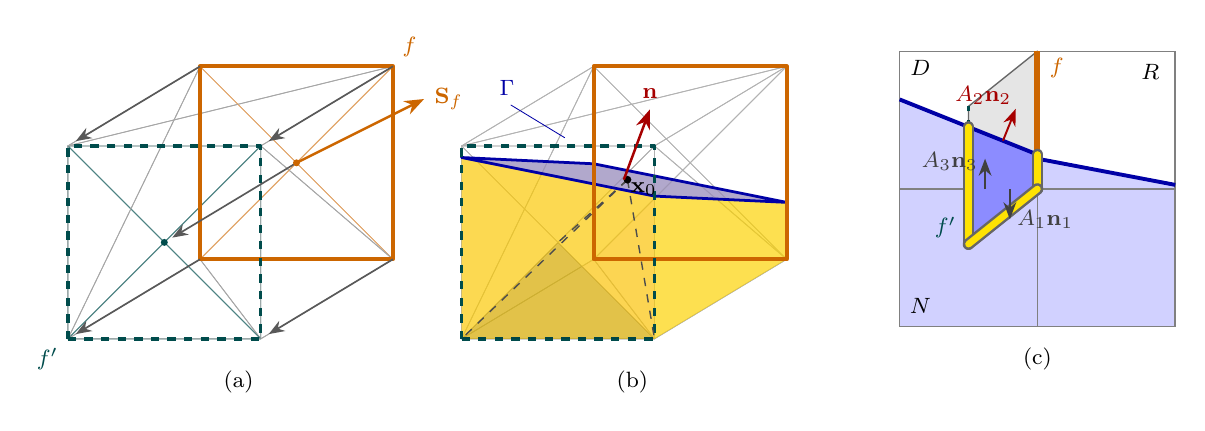
\begin{tikzpicture}[>=Stealth, font=\footnotesize, line join=round]
  \colorlet{facecol}{orange!80!black}
  \colorlet{precol}{teal!60!black}
  \colorlet{wetcol}{yellow!70!orange}
  \colorlet{capcol}{blue!55}
  \colorlet{ifacecol}{blue!65!black}
  \colorlet{fluidcol}{blue!18}
  \colorlet{gaincol}{blue!45}
  \colorlet{bdrycol}{black!50}
  % ------------------------------------------------ (a) the closed triangulation
  \begin{scope}[scale=2.45]
    % written by make_fig_sweptflux.py -- do not edit. d = (0.55, 0.3, 0.22), n = (0.28222, 0.18814, 0.94072), x0 = (0.75, 0.35, 0.5)
% signed volume 0.550000000000 (d.S_f = 0.550000000000), closure |sum a_T| = 0.0e+00, V^- = 0.339625000000, midpoint quadrature (160^3) 0.339625,
% cap area by closure 0.584658019700, by its polygon 0.584658019700
\draw[facecol!60, line width=0.3pt] (1.2000,0.8500) -- (0.7000,0.3500) -- (1.7000,0.3500) -- cycle;
\draw[precol!70, line width=0.3pt] (0.5150,0.4375) -- (1.0150,-0.0625) -- (0.0150,-0.0625) -- cycle;
\draw[black!35, line width=0.3pt] (0.7000,0.3500) -- (0.0150,-0.0625) -- (1.0150,-0.0625) -- cycle;
\draw[black!35, line width=0.3pt] (0.7000,0.3500) -- (1.0150,-0.0625) -- (1.7000,0.3500) -- cycle;
\draw[facecol!60, line width=0.3pt] (1.2000,0.8500) -- (1.7000,0.3500) -- (1.7000,1.3500) -- cycle;
\draw[precol!70, line width=0.3pt] (0.5150,0.4375) -- (1.0150,0.9375) -- (1.0150,-0.0625) -- cycle;
\draw[black!35, line width=0.3pt] (1.7000,0.3500) -- (1.0150,-0.0625) -- (1.0150,0.9375) -- cycle;
\draw[black!35, line width=0.3pt] (1.7000,0.3500) -- (1.0150,0.9375) -- (1.7000,1.3500) -- cycle;
\draw[facecol!60, line width=0.3pt] (1.2000,0.8500) -- (1.7000,1.3500) -- (0.7000,1.3500) -- cycle;
\draw[precol!70, line width=0.3pt] (0.5150,0.4375) -- (0.0150,0.9375) -- (1.0150,0.9375) -- cycle;
\draw[black!35, line width=0.3pt] (1.7000,1.3500) -- (1.0150,0.9375) -- (0.0150,0.9375) -- cycle;
\draw[black!35, line width=0.3pt] (1.7000,1.3500) -- (0.0150,0.9375) -- (0.7000,1.3500) -- cycle;
\draw[facecol!60, line width=0.3pt] (1.2000,0.8500) -- (0.7000,1.3500) -- (0.7000,0.3500) -- cycle;
\draw[precol!70, line width=0.3pt] (0.5150,0.4375) -- (0.0150,-0.0625) -- (0.0150,0.9375) -- cycle;
\draw[black!35, line width=0.3pt] (0.7000,1.3500) -- (0.0150,0.9375) -- (0.0150,-0.0625) -- cycle;
\draw[black!35, line width=0.3pt] (0.7000,1.3500) -- (0.0150,-0.0625) -- (0.7000,0.3500) -- cycle;
\draw[facecol, line width=1.4pt] (0.7000,0.3500) -- (1.7000,0.3500) -- (1.7000,1.3500) -- (0.7000,1.3500) -- cycle;
\draw[precol, line width=1.2pt, dashed] (0.0150,-0.0625) -- (1.0150,-0.0625) -- (1.0150,0.9375) -- (0.0150,0.9375) -- cycle;
\draw[->, black!65, line width=0.6pt] (0.7000,0.3500) -- (0.0561,-0.0378);
\draw[->, black!65, line width=0.6pt] (1.7000,0.3500) -- (1.0561,-0.0378);
\draw[->, black!65, line width=0.6pt] (1.7000,1.3500) -- (1.0561,0.9623);
\draw[->, black!65, line width=0.6pt] (0.7000,1.3500) -- (0.0561,0.9623);
\draw[->, black!65, line width=0.6pt] (1.2000,0.8500) -- (0.5561,0.4622);
\fill[facecol] (1.2000,0.8500) circle[radius=0.018];
\fill[precol] (0.5150,0.4375) circle[radius=0.018];
\coordinate (fC) at (1.2000,0.8500);
\coordinate (pC) at (0.5150,0.4375);
\coordinate (fS) at (1.5150,1.0075);
\coordinate (fP) at (1.7000,1.3500);
\coordinate (pP) at (0.0150,-0.0625);

    \draw[->, facecol, line width=0.9pt] (fC) -- ($(fC)!2.1!(fS)$) node[right=0pt] {$\mathbf{S}_f$};
    \node[facecol, anchor=south west] at (fP) {$f$};
    \node[precol, anchor=north east] at (pP) {$f'$};
    \node[anchor=north] at (0.9,-0.18) {(a)};
  \end{scope}
  % ------------------------------------------------ (b) the cut by the donor's plane
  \begin{scope}[xshift=5.0cm, scale=2.45]
    % written by make_fig_sweptflux.py -- do not edit. d = (0.55, 0.3, 0.22), n = (0.28222, 0.18814, 0.94072), x0 = (0.75, 0.35, 0.5)
% signed volume 0.550000000000 (d.S_f = 0.550000000000), closure |sum a_T| = 0.0e+00, V^- = 0.339625000000, midpoint quadrature (160^3) 0.339625,
% cap area by closure 0.584658019700, by its polygon 0.584658019700
\draw[black!30, line width=0.3pt] (1.2000,0.8500) -- (0.7000,0.3500) -- (1.7000,0.3500) -- cycle;
\draw[black!30, line width=0.3pt] (0.5150,0.4375) -- (1.0150,-0.0625) -- (0.0150,-0.0625) -- cycle;
\draw[black!30, line width=0.3pt] (0.7000,0.3500) -- (0.0150,-0.0625) -- (1.0150,-0.0625) -- cycle;
\draw[black!30, line width=0.3pt] (0.7000,0.3500) -- (1.0150,-0.0625) -- (1.7000,0.3500) -- cycle;
\draw[black!30, line width=0.3pt] (1.2000,0.8500) -- (1.7000,0.3500) -- (1.7000,1.3500) -- cycle;
\draw[black!30, line width=0.3pt] (0.5150,0.4375) -- (1.0150,0.9375) -- (1.0150,-0.0625) -- cycle;
\draw[black!30, line width=0.3pt] (1.7000,0.3500) -- (1.0150,-0.0625) -- (1.0150,0.9375) -- cycle;
\draw[black!30, line width=0.3pt] (1.7000,0.3500) -- (1.0150,0.9375) -- (1.7000,1.3500) -- cycle;
\draw[black!30, line width=0.3pt] (1.2000,0.8500) -- (1.7000,1.3500) -- (0.7000,1.3500) -- cycle;
\draw[black!30, line width=0.3pt] (0.5150,0.4375) -- (0.0150,0.9375) -- (1.0150,0.9375) -- cycle;
\draw[black!30, line width=0.3pt] (1.7000,1.3500) -- (1.0150,0.9375) -- (0.0150,0.9375) -- cycle;
\draw[black!30, line width=0.3pt] (1.7000,1.3500) -- (0.0150,0.9375) -- (0.7000,1.3500) -- cycle;
\draw[black!30, line width=0.3pt] (1.2000,0.8500) -- (0.7000,1.3500) -- (0.7000,0.3500) -- cycle;
\draw[black!30, line width=0.3pt] (0.5150,0.4375) -- (0.0150,-0.0625) -- (0.0150,0.9375) -- cycle;
\draw[black!30, line width=0.3pt] (0.7000,1.3500) -- (0.0150,0.9375) -- (0.0150,-0.0625) -- cycle;
\draw[black!30, line width=0.3pt] (0.7000,1.3500) -- (0.0150,-0.0625) -- (0.7000,0.3500) -- cycle;
\fill[wetcol, opacity=0.45] (1.1125,0.7625) -- (0.7000,0.3500) -- (1.7000,0.3500) -- (1.3313,0.7188) -- cycle;
\fill[wetcol!70!orange, opacity=0.45] (0.5150,0.4375) -- (1.0150,-0.0625) -- (0.0150,-0.0625) -- cycle;
\fill[wetcol, opacity=0.45] (0.7000,0.3500) -- (0.0150,-0.0625) -- (1.0150,-0.0625) -- cycle;
\fill[wetcol, opacity=0.45] (0.7000,0.3500) -- (1.0150,-0.0625) -- (1.7000,0.3500) -- cycle;
\fill[wetcol, opacity=0.45] (1.3312,0.7188) -- (1.7000,0.3500) -- (1.7000,0.6450) -- cycle;
\fill[wetcol!70!orange, opacity=0.45] (0.5150,0.4375) -- (0.7983,0.7208) -- (1.0150,0.6775) -- (1.0150,-0.0625) -- cycle;
\fill[wetcol, opacity=0.45] (1.7000,0.3500) -- (1.0150,-0.0625) -- (1.0150,0.6775) -- (1.3359,0.6623) -- cycle;
\fill[wetcol, opacity=0.45] (1.7000,0.3500) -- (1.3359,0.6623) -- (1.7000,0.6450) -- cycle;
\fill[wetcol!70!orange, opacity=0.45] (0.5150,0.4375) -- (0.0900,0.8625) -- (0.7983,0.7208) -- cycle;
\fill[wetcol, opacity=0.45] (0.7000,0.8450) -- (0.7000,0.3500) -- (1.1125,0.7625) -- cycle;
\fill[wetcol!70!orange, opacity=0.45] (0.5150,0.4375) -- (0.0150,-0.0625) -- (0.0150,0.8775) -- (0.0900,0.8625) -- cycle;
\fill[wetcol, opacity=0.45] (0.0150,0.8775) -- (0.0150,-0.0625) -- (0.4606,0.8564) -- cycle;
\fill[wetcol, opacity=0.45] (0.4606,0.8564) -- (0.0150,-0.0625) -- (0.7000,0.3500) -- (0.7000,0.8450) -- cycle;
\fill[capcol, opacity=0.55] (0.0900,0.8625) -- (0.0150,0.8775) -- (0.4606,0.8564) -- (0.7000,0.8450) -- (1.1125,0.7625) -- (1.3313,0.7188) -- (1.7000,0.6450) -- (1.3359,0.6623) -- (1.0150,0.6775) -- (0.7983,0.7208) -- cycle;
\draw[ifacecol, line width=1.0pt] (0.0900,0.8625) -- (0.0150,0.8775) -- (0.4606,0.8564) -- (0.7000,0.8450) -- (1.1125,0.7625) -- (1.3313,0.7188) -- (1.7000,0.6450) -- (1.3359,0.6623) -- (1.0150,0.6775) -- (0.7983,0.7208) -- cycle;
\draw[facecol, line width=1.4pt] (0.7000,0.3500) -- (1.7000,0.3500) -- (1.7000,1.3500) -- (0.7000,1.3500) -- cycle;
\draw[precol, line width=1.2pt, dashed] (0.0150,-0.0625) -- (1.0150,-0.0625) -- (1.0150,0.9375) -- (0.0150,0.9375) -- cycle;
\fill[black, opacity=0.10] (0.5150,0.4375) -- (1.0150,-0.0625) -- (0.0150,-0.0625) -- cycle;
\draw[black!70, dashed, line width=0.5pt] (0.8750,0.7625) -- (0.5150,0.4375);
\draw[black!70, dashed, line width=0.5pt] (0.8750,0.7625) -- (1.0150,-0.0625);
\draw[black!70, dashed, line width=0.5pt] (0.8750,0.7625) -- (0.0150,-0.0625);
\fill[black] (0.8750,0.7625) circle[radius=0.02];
\coordinate (xz) at (0.8750,0.7625);
\coordinate (capC) at (0.8559,0.7628);
\coordinate (capN) at (0.9909,1.1266);
\coordinate (tC) at (0.5150,0.1042);

    \draw[->, red!65!black, line width=0.9pt] (capC) -- (capN) node[above=0pt] {$\mathbf{n}$};
    \node[anchor=north west, inner sep=1pt] at (xz) {$\mathbf{x}_0$};
    \node[ifacecol, anchor=south] at (0.25,1.15) {$\Gamma$};
    \draw[ifacecol, line width=0.3pt] (0.27,1.15) -- (0.55,0.98);
    \node[anchor=north] at (0.9,-0.18) {(b)};
  \end{scope}
  % ------------------------------------------------ (c) the pieces, two-dimensional cut
  \begin{scope}[xshift=10.6cm, yshift=1.75cm, scale=1.75]
    % liquid: D below its plane, R below its own plane, the lower row full
    \fill[fluidcol] (0,-1) rectangle (2,0);
    \fill[fluidcol] (0,0) -- (1,0) -- (1,0.25) -- (0,0.65) -- cycle;
    \fill[fluidcol] (1,0) -- (2,0) -- (2,0.03) -- (1,0.22) -- cycle;
    \draw[bdrycol, line width=0.5pt] (0,-1) grid[step=1] (2,1);
    \draw[ifacecol, line width=1.4pt] (0,0.65) -- (1,0.25);
    \draw[ifacecol, line width=1.4pt] (1,0.22) -- (2,0.03);
    % the swept volume and its two pieces
    \fill[black!10] (1,0) -- (1,1) -- (0.5,0.6) -- (0.5,0) -- cycle;
    \fill[gaincol] (1,0) -- (1,0.25) -- (0.5,0.45) -- (0.5,0) -- cycle;
    \fill[gaincol] (1,0) -- (0.5,0) -- (0.5,-0.4) -- cycle;
    \draw[black!60, line width=0.5pt] (1,0) -- (1,1) -- (0.5,0.6) -- (0.5,-0.4) -- cycle;
    \draw[ifacecol, line width=1.4pt] (0.5,0.45) -- (1,0.25);
    % the wetted parts of the boundary of the swept volume and the face
    \draw[precol, line width=1.2pt, dashed] (0.5,-0.4) -- (0.5,0.6);
    \draw[facecol, line width=2.2pt] (1,0) -- (1,1);
    \draw[wetted] (0.5,-0.4) -- (0.5,0.45);
    \draw[wetted] (1,0) -- (1,0.25);
    \draw[wetted] (0.5,-0.4) -- (1,0);
    % the caps and their normals: the cell plane y = 0 (both pieces) and D's plane
    \draw[->, black!75, line width=0.7pt] (0.8,0.0) -- (0.8,-0.22) node[right=-1pt] {$A_1\mathbf{n}_1$};
    \draw[->, black!75, line width=0.7pt] (0.62,0.0) -- (0.62,0.22) node[left=-1pt, pos=0.9] {$A_3\mathbf{n}_3$};
    \draw[->, red!65!black, line width=0.7pt] (0.75,0.35) -- ++(0.0928,0.232) node[above left=-2pt] {$A_2\mathbf{n}_2$};
    \node at (0.15,0.88) {$D$};
    \node at (0.15,-0.85) {$N$};
    \node at (1.82,0.85) {$R$};
    \node[facecol, anchor=west] at (1.02,0.88) {$f$};
    \node[precol, anchor=east] at (0.48,-0.28) {$f'$};
    \node[anchor=north] at (1,-1.08) {(c)};
  \end{scope}
\end{tikzpicture}
\caption{The swept-face advection. (a) A face $f$ (orange) with its area vector $\mathbf{S}_f$, traced backward to its pre-image $f'$ (dashed) along the trajectories of its vertices and centre (arrows); the swept volume is closed by the face fan, the reversed pre-image fan and two triangles per lateral quadrilateral, $4F = 16$ triangles for a quadrilateral face. (b) The same volume cut by a plane with normal $\mathbf{n}$: the wetted parts of the triangles (gold), the cap $\Gamma$ (blue), and the cone from the point $\mathbf{x}_0$ of the plane to one wetted triangle (dashed), one term of \cref{eq:swept-volume}; drawn from the geometry computed by \texttt{make\_fig\_sweptflux.py}, whose closed form reproduces a quadrature of the liquid indicator. (c) A two-dimensional cut of the pieces: the swept volume of $f$ reaches from its donor $D$, an interface cell clipped by its own plane, into the full neighbour $N$, wet in total; each liquid piece is closed by the wetted parts of the swept volume's boundary (gold) and by its caps on the cell plane and on $D$'s plane, whose areas follow from the closure \cref{eq:swept-closure}. The wetted part of $f'$ gives $\alpha_f^{n+1} = 0.85$.}
\label{fig:sweptflux}
\end{figure}


The plane-clipped loop of the first preprint takes its volume flux from isoAdvector, which cuts the volume swept through a face by the donor's plane, extended beyond the donor where the swept volume leaves it (\cref{sec:oblique}), and its face fraction from a second operation, the sweep of the face by the moving plane. The swept-face advection computes both from one geometric object, the volume that a face sweeps over the step, traced backward from the face at $t^{n+1}$ and cut by the planes of the cells that this volume occupies at $t^n$. It needs four constructions, the trajectories of the face's points, a closed triangulation of the swept volume, the liquid volume of a triangulated polyhedron under a plane, and the decomposition of the swept volume into its pieces in the cells it reaches. The scheme is implemented in the branch \texttt{davof-swept} of the fork \citep{TwoPhaseFlowFork2026} (\texttt{fluxIntegration sweptFaceCells}). It uses planes only; the paraboloid dual advection of the first preprint keeps its prism flux.

\emph{Trajectories.} The vertices $\mathbf{p}_i$ and the centre $\x_f$ of a face at $t^{n+1}$ are traced backward to the pre-image $f'$ at $t^n$, with vertices $\mathbf{p}_i'$ and centre $\x_f'$, by the explicit midpoint rule
\begin{equation}
\x' = \x - \Delta t\,\mathbf{U}\big(\x - \tfrac12\Delta t\,\mathbf{U}(\x)\big),
\label{eq:swept-trace}
\end{equation}
second order in $\Delta t$, as in the face-vertex flux of \citet{MaricMarschallBothe2018}. The velocity at a vertex is OpenFOAM's volume-to-point interpolation; at the face centre and at the midpoint it is the cell-point interpolation, linear on the tetrahedra of the cell that contains the point, which is the donor or a cell of its vertex ring, otherwise found by a search. A midpoint outside the mesh takes the Euler step. For a uniform velocity the pre-image is $f - \mathbf{U}\Delta t$ and the swept volume is the prism of isoAdvector's kind.

\emph{The swept volume as a closed surface.} With the face and the pre-image triangulated as fans about their centres and every lateral quadrilateral split along a diagonal, the boundary of the swept volume $\Omega_f$ of a face with $F$ vertices is the closed list of $4F$ planar triangles (\cref{fig:sweptflux}a)
\begin{equation}
(\x_f, \mathbf{p}_i, \mathbf{p}_{i+1}), \quad
(\x_f', \mathbf{p}_{i+1}', \mathbf{p}_i'), \quad
(\mathbf{p}_i, \mathbf{p}_i', \mathbf{p}_{i+1}'), \quad
(\mathbf{p}_i, \mathbf{p}_{i+1}', \mathbf{p}_{i+1}), \qquad i = 1, \ldots, F .
\label{eq:swept-triangles}
\end{equation}
With $\Sf$ pointing from the owner to the neighbour, the list is outward for $\phi_f = \mathbf{U}_f\cdot\Sf > 0$, when the swept volume lies on the owner's side, and every triangle is reversed for $\phi_f < 0$. The signed volume $\tfrac16\sum_T \mathbf{p}_T\cdot(\mathbf{q}_T\times\mathbf{r}_T)$ of the vertices $\mathbf{p}_T$, $\mathbf{q}_T$, $\mathbf{r}_T$ of the triangles confirms the orientation; a list with a negative volume is reversed and counted. Warped faces, twisted lateral quadrilaterals and non-convex swept volumes are represented by the same list, which is closed by construction, $\sum_T \mathbf{a}_T = \mathbf{0}$ for the area vectors $\mathbf{a}_T$ of the triangles.

\emph{The liquid volume under a plane.} Let the plane $(\x - \x_0)\cdot\n = 0$ bound the liquid $(\x - \x_0)\cdot\n \le 0$, and let $\mathbf{a}_T^-$ be the area vector of the wetted part $T^-$ of triangle $T$, the polygon that one clip of $T$ against the plane leaves. The liquid part of $\Omega_f$ is bounded by the wetted parts and by the cap $\Gamma$ on the plane (\cref{fig:sweptflux}b). On a planar triangle $(\x - \x_0)\cdot\n_T$ is constant, and on the cap $(\x - \x_0)\cdot\n$ vanishes, so the divergence theorem for $\x - \x_0$ on the liquid part gives
\begin{equation}
V_f^- = \frac13\sum_T (\mathbf{p}_T - \x_0)\cdot\mathbf{a}_T^- ,
\label{eq:swept-volume}
\end{equation}
with $\mathbf{p}_T$ any vertex of $T$. The volume is the sum of the signed cones from a point of the plane to the wetted triangles, the form in which hydrostatics computes the displaced volume of a hull below the waterline, and the cap is never constructed. Its area and its first moment follow from the same clips, by the closure of the liquid part's boundary and by the divergence theorem for $\x\otimes\mathbf{e}_j$,
\begin{equation}
|\Gamma| = -\,\n\cdot\sum_T \mathbf{a}_T^- , \qquad
\int_\Gamma \x\,dS = V_f^-\,\n - \sum_T (\n\cdot\n_T)\int_{T^-}\x\,dS ,
\label{eq:swept-cap}
\end{equation}
so the area and the centroid of the interface polygon inside the swept volume are available without assembling it. \Cref{eq:swept-volume} is the position identity \cref{eq:avof-identities} read in the other direction: there the volume and the wetted face areas fix the plane, here the plane fixes the wetted areas and the volume. The truncation of non-convex polyhedra from face quantities, without the connectivity of the truncated body, is established for the positioning problem by \citet{KromerBothe2022} and in VOFTools~5 \citep{LopezEtAl2020VOFTools5}; \cref{eq:swept-volume} is its one-level case on a boundary that is already triangulated. It replaces the decomposition of the swept volume into tetrahedra clipped one by one, which needs an apex and the signs of the tetrahedra of a twisted volume. For the swept volume of \cref{fig:sweptflux}b it reproduces a quadrature of the liquid indicator, and the cap area by closure equals the area of the cap polygon.

\emph{The pieces.} The pre-image leaves the donor whenever the displacement has a component along the face; in the rotation test below every pre-image does. Cutting the whole swept volume by the donor's plane then uses that plane outside the cell whose volume fraction positioned it (\cref{sec:oblique}). The swept volume is therefore split into its pieces $\Omega_f\cap\Omega_c$ in the donor and in the cells $c$ of the donor's vertex ring, the cells that share a vertex with it, and each piece takes the liquid of its own cell at $t^n$ (\cref{fig:sweptflux}c). A piece is wet in total in a full cell, dry in an empty one ($\alpha_c = 0$), and clipped by the cell's own plane in an interface cell. A partial cell without a plane of its own, a wisp, typically a cell whose corner the interface cuts so that its area vector falls below the interface threshold, is clipped by the plane of its closest face neighbour with a plane where that plane puts the wisp's liquid $\alpha_c|\Omega_c|$ into it to $10^{-9}|\Omega_c|$, and otherwise by the neighbour's normal with the plane positioned in the wisp by $\alpha_c$. The neighbour's plane alone is not enough, because extended into a wisp of a curved interface it can hold more liquid than the wisp has, and it left the rotation of \cref{sec:ladders} unbounded ($\min\alpha = -1.7\cdot10^{-5}$ at $N = 64$); the positioned plane alone is not either, because the face fraction of a corner grows as $\alpha_c^{2/3}$, so that a volume fraction at round-off becomes a visible face fraction. Every face whose swept volume touches a partial cell is computed by the swept flux, because a face that keeps the algebraic upwind flux outside the band of the interface cells carries liquid its swept volume does not hold; a wall face among them keeps the flux of the boundary condition where that condition fixes $\alpha$, since a piece computed through a wall fixed at zero would carry liquid out of the domain. The piece is $\Omega_f$ intersected with the half-spaces of the cell's face planes and, in an interface cell, with its liquid half-space. Its boundary consists of the boundary triangles of $\Omega_f$ clipped by these half-spaces, one plane at a time by the polygon clip of \citet{SutherlandHodgman1974}, and of one cap on every plane that cuts it. On cap $i$, with outward unit normal $\n_i$ and area $A_i$, $\x\cdot\n_i$ is the constant $\x_{0,i}\cdot\n_i$, and the closure of the piece's boundary,
\begin{equation}
\sum_T \mathbf{a}_T^{\cap} + \sum_{i=1}^{k} A_i\,\n_i = \mathbf{0} ,
\label{eq:swept-closure}
\end{equation}
with $\mathbf{a}_T^{\cap}$ the area vectors of the clipped triangles, is three equations for the $k$ cap areas, solved in least squares for $k \le 3$ independent normals. The divergence theorem for $\x$ then gives the liquid volume of the piece and the flux of the face,
\begin{equation}
V_c^- = \frac13\Big[\sum_T \mathbf{p}_T\cdot\mathbf{a}_T^{\cap} + \sum_{i=1}^{k} A_i\,(\x_{0,i}\cdot\n_i)\Big], \qquad
V_f^- = \sum_c V_c^- .
\label{eq:swept-piece}
\end{equation}
A face-neighbour piece of an interface cell has one cell plane and the cell's own plane, an edge-neighbour piece two cell planes and its own plane, so three caps suffice within one layer of cells. A piece with more than three caps, or with a plane parallel to a cell face, makes the face fall back to the clip of the whole swept volume by the donor's plane (counted). Which planes carry a cap is read from the final clipped polygons: a plane carries a cap when it produced an edge of a final wet polygon, the edges being labelled through the clips, and a boundary triangle lying in a cell plane is a contact, dropped from the piece, when the donor lies on the other side of that plane. With these two rules the cap set is a property of the piece, independent of the order in which a cell's faces are clipped, an order that differs between a serial and a decomposed mesh.

\emph{The correction of the swept volume to the flux volume.} Under a non-uniform velocity the traced volume $V_g = \tfrac13\sum_T \x_T\cdot\mathbf{a}_T$ of the closed list, the sum of \citet{TolleEtAl2022TriSurface}, differs from the flux volume $V_f = |\phi_f|\Delta t$, with $\phi_f$ taken at the half step, the temporal pair of the midpoint trace \cref{eq:swept-trace}; under rotation by about $(\omega\Delta t)^2/12$ relative, so that a wholly wet swept volume would carry more liquid out of a full cell than its upwind flux. The correction of the unsplit face-vertex flux of \citet{MaricMarschallBothe2018} removes the difference: only the face points are traced, the apex of the pre-image fan starts at the mean of the traced vertices and is moved along the pre-image's outward area vector $\mathbf{A}_{f'}$ by $\delta = 3\,(V_f - V_g)/|\mathbf{A}_{f'}|$, which is exact because the volume of the list is linear in the apex and the fan's area vector does not depend on it, and the corrected list is clipped and capped as before; no tetrahedra or prisms are formed. The alternative that scales the liquid by $V_f/V_g$ divides by $V_g$, which vanishes for a face twisted near a rotation axis, whereas the pyramid divides by $|\mathbf{A}_{f'}|$ only. Under uniform translation the correction is at round-off; under rotation at an OpenFOAM Courant number of $0.86$ to $0.88$ (\cref{sec:ladders}) the defect $|V_f - V_g|/V_f$ reaches $1.4\cdot10^{-5}$ to $8\cdot10^{-7}$, no swept volume is twisted, also not at the poles of a pure spin, and the two corrections agree in every error norm within $10^{-6}$ relative: on these cases at OpenFOAM Courant numbers up to one they are indistinguishable.

\emph{The face update.} The pieces of the pre-image fan, clipped by the same half-spaces, give the wetted area vector $\mathbf{a}_{f'}^-$ of the pre-image, for which no caps are needed, and the new face fraction
\begin{equation}
\alpha_f^{n+1} = \frac{\mathbf{a}_{f'}^-\cdot\mathbf{A}_{f'}}{|\mathbf{A}_{f'}|^2} ,
\label{eq:swept-face}
\end{equation}
with $\mathbf{A}_{f'}$ the area vector of the pre-image, which is the semi-Lagrangian update \cref{eq:face-update} evaluated with the clips of the flux. A part of a pre-image that lies in a cell plane, as on a face parallel to the velocity, belongs to the cell on the donor's side of that plane; counted on both sides, it gave such a face the sum of two fractions.

\emph{Conservation, boundedness and parallel evaluation.} The flux volume carries the sign of $\phi_f$ and is the same for both cells of the face, so the liquid volume is conserved by antisymmetry. Boundedness is not built in, because \cref{eq:swept-piece} does not limit the flux by the liquid the donor holds; the bounding step of the isoAdvector framework is kept unchanged, and \cref{sec:results} reports the bounds measured. In parallel, the cells of a vertex ring that lie on another processor are fetched once per step through OpenFOAM's zoneDistribute stencil \citep{ScheuflerRoenby2019} and one transfer of the packed cells, with their volume fractions, planes, face planes, bounding boxes and the tetrahedra and point velocities of the cell-point interpolation, so that a piece or a midpoint in a remote cell is computed from the numbers the serial run uses. A processor face is computed on the rank of its donor and copied to the other side; only the order of the summands differs from serial.

\emph{The reference setting.} The rules above entered the fork in steps, each as an opt-in key verified against the build before it, and since commit \texttt{407f969} they are the defaults: the wisp rule with its match tolerance of $10^{-9}$ and no empty band, the computed band with its wall faces, the pyramid correction, the plane positioned by consecutive cubic splines with the volume anchor of the surface skipped where the plane is already within its tolerance, a pre-test that skips the ring cells the swept volume only touches, and a per-step cache of the traced points. The last two reproduce the clips bit for bit and are cost measures (\cref{sec:efficiency}). With no key in the dictionary this setting reproduces the plane gate's verdicts and round-off maxima, the transported fields of the rotation and the lines within $1.4\cdot10^{-6}$ in the shape error and the face fractions and within $0.62\,\%$ in the centroid, the parallel identity, bounded ($\min\alpha \ge -6.6\cdot10^{-11}$, excess at most $6.2\cdot10^{-10}$) and conservative to $10^{-11}\,\%$, at $2.1$ to $2.8$ times less wall clock than the comparison of \cref{sec:cmp}. The results below name the setting they were computed with.

\emph{Scope and limits.} The closed forms \cref{eq:swept-volume,eq:swept-piece} need $\x\cdot\n$ constant on every cap, so the scheme is for planes only. A paraboloid or a sphere as a cell's surface is rejected; the curved surface of the first preprint keeps its prism flux with the volume rule of \citet{KromerBothe2023Init}. The pieces cover one layer of cells around the donor, which contains the swept volume while the displacement per step stays below one cell size along each axis; a part beyond it is skipped and counted. The measurements reach an OpenFOAM Courant number of one on the translated plane and in the comparison of \cref{sec:cmp}, and $0.86$ to $0.88$ under rotation (\cref{sec:ladders}); above an OpenFOAM Courant number between $1.05$ and $1.29$ the plane is not kept, and under rotation at $2.2$ parts of the swept volumes leave the one layer and $\alpha$ reaches $-1.7\cdot10^{-4}$ at $N = 128$. The cells are assumed convex, and the scheme has been run on Cartesian hexahedra only. The cost is the main limitation: at the same number of ranks the swept-face advection takes $3$ to $10$ times the wall clock of plicRDF with isoAdvector in the registered comparison, and $1.9$ times plicRDF's serial step after the optimisation of \cref{sec:efficiency}. The closure residual of the accepted pieces, whose largest value per step lies between $10^{-11}$ and $10^{-6}$, is above round-off for some pieces, which have not been identified.

\section{Cases, measures and comparators}
\label{sec:cases}

Every case runs in the TwoPhaseFlow fork on Cartesian hexahedra with the velocity prescribed. The \emph{translated plane} is the plane of the first preprint, with the normal $(0.3, 0.5, 0.8124)$ through $(2.13, 1.71, 1.97)\,\mathrm{mm}$ in an $8^3$ box of $4\,\mathrm{mm}$ side, carried over $0.2L$ along its normal (the normal arm) and along $(1, 0, 0)$ (the oblique arm), $N = 20$ to $160$ cells per side, from its exact cell and face fractions; the gate is that the face fractions and the normal stay at round-off, $10^{-12}$ in $L_1$, over the run. The \emph{sphere} has $R = 0.15$ in a $2 \times 1 \times 1$ box with $N$ cells across the box height, $R/h = 4.8$ to $19$ at $N = 32$ to $128$. It is translated along $x$ by $\mathbf{U} = (1, 0, 0)$ over one box length (the \emph{axis-aligned translation}), translated along $x$ and along the $x$--$z$ diagonal at $|\mathbf{U}| = \pi/2$ over $t = 0.45$ (the \emph{lines}), and turned once about the axis parallel to $y$ through $(0.75, \cdot, 0.5)$ with $\omega = 2\pi$ from its centre at $(0.5, 0.5, 0.5)$ (the \emph{rotation}), in which every pre-image leaves its donor. The initial state is the \emph{exact state} of the sphere, the exact cell and face fractions, except for the axis-aligned translation ladder, which starts from the \emph{DA-Q state} of the first preprint, the Detrixhe--Aslam cell fractions with quadratic face fractions, $7.28\cdot10^{-6}\,\mathrm{m^3}$ off the exact sphere at $N = 128$, so that its rows compare with the plane-clipped loop's. The volume fraction is fixed at zero on the walls of the sphere cases.

Two Courant numbers appear. The \emph{target} Courant number of a case sets the time step from a reference speed, $|\mathbf{U}|$ on the lines and the speed of the sphere's far point under rotation. \emph{OpenFOAM's} Courant number is the maximum over the cells of half the sum of $|\phi_f|\Delta t$ over the cell volume; under uniform translation it is the sum of the displacements per step along the three axes over $h$, equal to the target along $x$, $1.61$ times it on the plane's normal arm and $\sqrt{2}$ times it on the diagonal, and under rotation it is reached at the corners of the box, $0.86$, $0.87$ and $0.88$ for the target $0.2$ at $N = 32$, $64$, $128$. Both are given where a case is cited.

The errors at the end of a run are $L_1(\alpha_f)$, the face-fraction error as a fraction over the faces of the interface cells against the exact state; $L_1(\mathbf{x})$ and $L_1(\mathbf{n})$, the centroid and normal errors of the recovered planes against the exact body; $E_{\mathrm{shape}} = \sum_k|\alpha_k - \alpha_k^{\mathrm{ex}}|\,|\Omega_k|$ in $\mathrm{m^3}$ against the exact sphere--box cell fractions (the sphere's volume is $1.41\cdot10^{-2}\,\mathrm{m^3}$); and on the lines $E_c$, the mean of $|\alpha_k - \alpha_k^{\mathrm{ex}}|$ over the exact interface cells. Boundedness is the minimum of $\alpha$ and its largest excess over one after the bounding step, over the whole run; conservation is the relative change of $\sum_k \alpha_k|\Omega_k|$. Orders are least-squares slopes over $N = 32$, $64$, $128$ unless stated. The comparator is plicRDF with isoAdvector of OpenFOAM's \texttt{geometricVoF} library \citep{ScheuflerRoenby2019,ScheuflerRoenby2023TwoPhaseFlow} on the same initial $\alpha_k$, mesh, time step and ranks, with the settings of the fork's advection test suite where stated: no snapping, no clipping, one correction, three bounding passes on the translations and five on the rotation. The second comparator is the plane-clipped loop of the first preprint, the DAVOF reconstruction with isoAdvector's flux and the plane face update. Wall-clock times are the median of three repetitions of a case on one exclusive node of two Intel Xeon Platinum 9242 processors (48 cores each), the methods in rotated order and the diagnostics at the end of the run only, for every method alike.

\section{Results}
\label{sec:results}

\subsection{The translated plane}
\label{sec:planegate}

The translated plane tests the pieces, because every piece of a plane case is cut by the same plane. With the earlier rules the swept-face advection did not keep it. From the second step on, the pieces in wisps, taken wet or dry or counted empty below $10^{-8}$, left face-fraction errors up to $6\cdot10^{-6}$ at a target Courant number of $0.2$, and at $0.95$ the faces outside the computed band left errors of $0.1$. With the wisp rule and the computed band of \cref{sec:method} it was run in 64 cases, $N = 20$ to $160$, target Courant numbers $0.2$, $0.5$, $0.8$ and $0.95$ of $|\mathbf{U}|\Delta t/h$, both arms, exact and ring normal. Every case with an OpenFOAM Courant number of at most one keeps the face fractions and the normal to $10^{-11}$ in $L_1$, is bounded to $-8.2\cdot10^{-13}$, and has a shape error below $7.1\cdot10^{-12}$ of the liquid volume. The round-off gate of $10^{-12}$ holds at $N \le 40$ in 23 of 24 such cases and at $N = 80$ and $160$ in 6 of 24: there a floor of the pieces grows with $N$, to $9.5\cdot10^{-12}$ at $N = 160$, while the prism and the one-donor flux keep the same cases at $2.4\cdot10^{-13}$; its cause is open. On the normal arm at the targets $0.8$ and $0.95$, OpenFOAM Courant numbers of $1.29$ and $1.53$, the minimum of $\alpha$ grows by a factor of about $1.4$ per step, to $-4.3\cdot10^{-4}$ at $N = 160$; at $1.05$ it stays at round-off in a 24-step run at $N = 80$, so the scheme is not yet usable above an OpenFOAM Courant number between $1.05$ and $1.29$, for a reason that is open. On the rotation and on the translated sphere at $N = 32$ and $64$ the rules change every error by less than $8\cdot10^{-4}$ relative, and the runs stay bounded and conservative. The one-donor form of the scheme, which clips the whole swept volume by the donor's plane without the pieces, holds the gate at round-off in every run and reproduces the prism flux on the translated sphere with the exact normal to $3\cdot10^{-12}$ at $N = 32$ and $64$; under rotation it is not bounded (\cref{sec:ladders}).

\subsection{The rotated and the translated sphere}
\label{sec:ladders}

Rotation is the test in which every pre-image leaves its donor. The sphere is turned once at a target Courant number of $0.2$ for its far point, OpenFOAM Courant number $0.86$ to $0.88$, in 400, 800 and 1600 steps at $N = 32$, $64$ and $128$, from the exact state, with the plane of every interface cell positioned by $\alpha_k$ with the exact or the ring normal, the scaling as the volume correction, the earlier wisp rule, and $N = 128$ on 64 ranks. Every run completes the turn bounded and conservative, without a fallback to the one-donor clip (\cref{tab:swept-rotation}). With the same planes, the two fluxes that cut the whole swept volume by the donor's plane, the one-donor form of the scheme and the prism flux of the first preprint, leave the volume fraction unbounded at $N = 64$ ($\alpha$ down to $-0.18$ to $-0.28$ when the runs are stopped), and the prism flux also at $N = 128$. Over $N = 32$ to $128$ the face fractions converge below first order over the turn, at $0.68$ with the exact normal and $0.83$ with the ring normal, the centroid of the recovered planes at $1.71$ and $1.90$, and the shape error at $1.68$ and $1.86$. plicRDF with isoAdvector on the same rotation converges at $1.96$ in the centroid and $1.90$ in the shape error; at $N = 128$ both swept rows lie below its errors, at lower orders. Its run at $N = 128$, on 64 ranks like the swept ones, is not bounded with three bounding passes ($\min\alpha = -3.1\cdot10^{-5}$, excess $7.1\cdot10^{-7}$) and bounded with five (\cref{sec:cmp}), while its serial runs at $N = 32$ and $64$ stay within $-7.6\cdot10^{-13}$. In the first run of this ladder a face update from the donor's plane alone gave the end values of \cref{eq:swept-face} to $1\,\%$, so the per-turn order of the face fractions belongs to the loop of flux and planes. The face-fraction error grows about linearly over the turn, at a rate whose own order under refinement is about $0.45$ between $N = 32$ and $64$; \cref{sec:oblique} measures the corresponding build-up under straight oblique travel.

On the axis-aligned translation, from the DA-Q state at target Courant numbers $0.1$, $0.2$ and $0.5$ (OpenFOAM's definition gives the same number along one axis) and $N = 32$ to $128$ (on 64 ranks at $N = 128$), the swept-face advection gives the centroid and shape errors of the plane-clipped loop with either normal, to three digits at $\mathrm{Co} = 0.1$ and $0.2$ and within $1\,\%$ at $0.5$, and face fractions at or below the plane-clipped loop's at every Courant number, $2.7$ times lower with the exact normal and $1.8$ times lower with the ring normal at $\mathrm{Co} = 0.5$ (\cref{tab:swept-sphere}). With the ring normal at $\mathrm{Co} = 0.2$ its shape and centroid errors at $N = 128$ are $0.986$ and $0.987$ of plicRDF's; with the exact normal they are below plicRDF's. All 18 runs are bounded ($\min\alpha \ge -1.0\cdot10^{-12}$, excess at most $5.0\cdot10^{-11}$), conservative to $2.9\cdot10^{-12}\,\%$ and without a fallback.

The decomposed runs reproduce the serial one. On the rotation at $N = 32$, decompositions into 2, 4, 8 and 16 ranks differ from the serial run over 20 steps by at most $2.5\cdot10^{-12}$ in the volume fractions and $6.1\cdot10^{-12}$ in the face fractions, and every face of the serial run has a value in every decomposition; before the order-independent cap set, one face on 16 ranks took the pieces at step 20 where the serial run fell back. At $N = 128$, $4.2\cdot10^6$ cells, the advection call of a step takes $3.3\,\mathrm{s}$ in serial and $0.34$ to $0.36\,\mathrm{s}$ on 64 ranks, $9.6$ times less; a whole step of the 10-step run on which this was measured fell from $8.9$ to $0.49\,\mathrm{s}$, 18 times, because $5.6\,\mathrm{s}$ of its serial step were per-step diagnostics on two million cells that parallelise completely. The exchange proper takes 2 to $5\,\%$ of the advection call; the advection does not scale beyond 8 ranks because the interface band lies in a few ranks of the mesh-wide decomposition (\cref{sec:efficiency}).

\begin{table}[htbp]
\centering
\caption{The swept-face advection under rotation: the sphere turned once, target Courant number $0.2$ at its far point (OpenFOAM Courant number $0.86$ to $0.88$), exact initial state, the plane positioned by $\alpha_k$ (fork commit \texttt{1f3f238}, the earlier wisp rule and the scaling; $N = 128$ on 64 ranks), next to plicRDF with isoAdvector on the same rotation with three bounding passes. Errors at the end of the turn and the least-squares order $p$ over $N = 32$, $64$, $128$; $E_{\mathrm{shape}}$ in $\mathrm{m^3}$ against the exact sphere. The swept runs stay within $\alpha \ge -8.0\cdot10^{-13}$ and an excess over one of at most $8.2\cdot10^{-11}$ after the bounding, the liquid volume changes by at most $6.3\cdot10^{-12}\,\%$, and no face falls back to the one-donor clip. From \texttt{data/swept/itemC\_rotation\_ladder.csv}.}
\label{tab:swept-rotation}
\footnotesize
\begin{tabular}{llrrrr}
\toprule
method & error & $N = 32$ & $N = 64$ & $N = 128$ & $p$ \\
\midrule
swept-face, exact normal & $L_1(\alpha_f)$ & 2.31e-02 & 1.45e-02 & 8.94e-03 & 0.68 \\
 & $L_1(\mathbf{x})$ & 1.49e-03 & 4.72e-04 & 1.39e-04 & 1.71 \\
 & $E_{\mathrm{shape}}$ & 4.00e-04 & 1.29e-04 & 3.87e-05 & 1.68 \\
swept-face, ring normal & $L_1(\alpha_f)$ & 4.16e-02 & 2.32e-02 & 1.32e-02 & 0.83 \\
 & $L_1(\mathbf{x})$ & 2.81e-03 & 7.59e-04 & 2.02e-04 & 1.90 \\
 & $E_{\mathrm{shape}}$ & 7.60e-04 & 2.11e-04 & 5.74e-05 & 1.86 \\
plicRDF with isoAdvector & $L_1(\mathbf{x})$ & 3.48e-03 & 8.64e-04 & 2.31e-04 & 1.96 \\
 & $E_{\mathrm{shape}}$ & 9.00e-04 & 2.42e-04 & 6.44e-05 & 1.90 \\
\bottomrule
\end{tabular}
\end{table}

\begin{table}[htbp]
\centering
\caption{The swept-face advection on the axis-aligned translation of the sphere, from the DA-Q initial state, $N = 32$, $64$, $128$ ($N = 128$ on 64 ranks): errors at $N = 128$ with the least-squares orders $p$ over the three meshes, the face-fraction error of the plane-clipped loop with the same normal for comparison, and plicRDF on the same state. $E_{\mathrm{shape}}$ in $\mathrm{m^3}$ includes the $7.28\cdot10^{-6}\,\mathrm{m^3}$ by which the initial state lies off the exact sphere. The plane-clipped loop's $L_1(\mathbf{x})$ and $E_{\mathrm{shape}}$ equal the swept rows' to three digits at $\mathrm{Co} = 0.1$ and $0.2$ and within $1\,\%$ at $0.5$. From \texttt{data/swept/itemD\_comparison.csv}.}
\label{tab:swept-sphere}
\footnotesize
\setlength{\tabcolsep}{4pt}
\begin{tabular}{llrrrrrrr}
\toprule
Co & method & $L_1(\alpha_f)$ & $p$ & plane-clipped $L_1(\alpha_f)$ & $L_1(\mathbf{x})$ & $p$ & $E_{\mathrm{shape}}$ & $p$ \\
\midrule
0.1 & swept-face, exact & 3.72e-03 & 0.87 & 3.84e-03 & 7.93e-05 & 1.92 & 1.59e-05 & 1.90 \\
 & swept-face, ring & 7.67e-03 & 0.79 & 7.72e-03 & 1.34e-04 & 1.86 & 3.34e-05 & 1.82 \\
 & plicRDF & -- & -- & -- & 1.40e-04 & 1.90 & 3.43e-05 & 1.89 \\
0.2 & swept-face, exact & 2.96e-03 & 0.86 & 3.32e-03 & 6.75e-05 & 1.93 & 1.29e-05 & 1.90 \\
 & swept-face, ring & 5.56e-03 & 0.83 & 5.76e-03 & 1.02e-04 & 1.86 & 2.44e-05 & 1.84 \\
 & plicRDF & -- & -- & -- & 1.04e-04 & 1.94 & 2.48e-05 & 1.93 \\
0.5 & swept-face, exact & 1.28e-03 & 0.98 & 3.46e-03 & 4.75e-05 & 1.98 & 7.30e-06 & 1.93 \\
 & swept-face, ring & 1.62e-03 & 1.12 & 2.96e-03 & 4.88e-05 & 2.00 & 7.34e-06 & 2.04 \\
 & plicRDF & -- & -- & -- & 4.87e-05 & 1.99 & 7.96e-06 & 1.94 \\
\bottomrule
\end{tabular}
\end{table}

\subsection{Oblique translation: the build-up of the volume-fraction error}
\label{sec:oblique}

% The oblique excess on an equidistant Cartesian mesh (two-dimensional cut, cell size h = 1).
% Interface: the circle with centre (0.818, 0.4) and radius 1.72, liquid inside. The plane of
% every interface cell is n.x = c with the exact normal at the midpoint of the cell's arc and c
% positioned by the cell's exact liquid fraction (computed on Lichtenberg; values below):
%   cell (0,1) alpha 0.99230  n (-0.42208, 0.90656) c 1.73636
%   cell (0,2) alpha 0.07211  n (-0.13452, 0.99091) c 1.98602
%   cell (1,1) alpha 0.91710  n ( 0.53689, 0.84365) c 2.48705   (N, the lateral neighbour)
%   cell (1,2) alpha 0.02960  n ( 0.23864, 0.97111) c 2.29799   (D1)
%   cell (2,0) alpha 0.51042  n ( 0.99815, 0.06075) c 2.53616
%   cell (2,1) alpha 0.16289  n ( 0.83382, 0.55204) c 2.60692   (D2; the donor D in panel a)
% The jump of N's and D2's planes on x = 2: z = 1.6752 (N) and 1.7015 (D2).
% Displacement per step: 0.56h along x (a), 0.4h per axis (b); the measured runs: 0.126h.
% Panels (c, d): the measured E_c of the studies sphereRotation3D_hexFineLine{Diag,X}{RingSwept,RDF},
% column 10 of staticFaceFractions.dat, copied from the cluster into data/oblique.
\begin{figure}[tb]
\centering
% the half-plane n.x <= c and the line n.x = c, for a clip
\newcommand{\obqHalf}[3]{({#3*#1-20*#2},{#3*#2+20*#1}) -- ({#3*#1+20*#2},{#3*#2-20*#1})
  -- ({(#3-20)*#1+20*#2},{(#3-20)*#2-20*#1}) -- ({(#3-20)*#1-20*#2},{(#3-20)*#2+20*#1}) -- cycle}
\newcommand{\obqLine}[3]{({#3*#1-20*#2},{#3*#2+20*#1}) -- ({#3*#1+20*#2},{#3*#2-20*#1})}
% the liquid inside the circle, clipped to the mesh
\newcommand{\obqLiquid}{%
  \begin{scope}
    \clip (0,0) rectangle (4,4);
    \fill[fluidcol] (0.818,0.4) circle[radius=1.72];
  \end{scope}}
% the interface and every cell's plane
\newcommand{\obqPlanes}{%
  \begin{scope}
    \clip (0,0) rectangle (4,4);
    \draw[ifacecol!55, line width=0.5pt] (0.818,0.4) circle[radius=1.72];
  \end{scope}
  \foreach \ci/\cj/\nx/\nz/\cc in {0/1/-0.42208/0.90656/1.73636, 0/2/-0.13452/0.99091/1.98602,
      1/1/0.53689/0.84365/2.48705, 1/2/0.23864/0.97111/2.29799,
      2/0/0.99815/0.06075/2.53616, 2/1/0.83382/0.55204/2.60692}{%
    \begin{scope}
      \clip (\ci,\cj) rectangle ++(1,1);
      \draw[ifacecol, line width=1.5pt] \obqLine{\nx}{\nz}{\cc};
    \end{scope}}}
% panel (b): the swept volumes of f1 and f2, their cuts and the faces
\newcommand{\obqCorner}{%
  \fill[sweptcol] (2,2) -- (2,3) -- (1.6,2.6) -- (1.6,1.6) -- cycle;
  \fill[sweptcol] (2,2) -- (3,2) -- (2.6,1.6) -- (1.6,1.6) -- cycle;
  \begin{scope}
    \clip (2,1.6) -- (2.6,1.6) -- (3,2) -- (2,2) -- cycle;
    \fill[gaincol] \obqHalf{0.83382}{0.55204}{2.60692};
  \end{scope}
  \begin{scope}
    \clip (1.6,1.6) -- (2,2) -- (1.6,2) -- cycle;
    \fill[mismcol] \obqHalf{0.23864}{0.97111}{2.29799};
    \fill[gaincol] \obqHalf{0.53689}{0.84365}{2.48705};
    \draw[ifacecol, dashed, line width=0.9pt] \obqLine{0.23864}{0.97111}{2.29799};
  \end{scope}
  \begin{scope}
    \clip (1.6,1.6) -- (2,1.6) -- (2,2) -- cycle;
    \fill[mismcol] \obqHalf{0.83382}{0.55204}{2.60692};
    \fill[gaincol] \obqHalf{0.53689}{0.84365}{2.48705};
    \draw[ifacecol, dashed, line width=0.9pt] \obqLine{0.83382}{0.55204}{2.60692};
  \end{scope}
  \begin{scope}
    \clip (1,1) rectangle (2,2);
    \draw[ifacecol, line width=1.5pt] \obqLine{0.53689}{0.84365}{2.48705};
  \end{scope}
  \begin{scope}
    \clip (2,1) rectangle (3,2);
    \draw[ifacecol, line width=1.5pt] \obqLine{0.83382}{0.55204}{2.60692};
  \end{scope}
  \draw[black!55, line width=0.5pt] (2,2) -- (2,3) -- (1.6,2.6) -- (1.6,1.6) -- cycle;
  \draw[black!55, line width=0.5pt] (2,2) -- (3,2) -- (2.6,1.6) -- (1.6,1.6);
  \draw[black!55, line width=0.4pt, densely dotted] (1.6,1.6) -- (2,2);
  \draw[facecol, line width=2.6pt] (2,2) -- (2,3);
  \draw[facecol, line width=2.6pt] (2,2) -- (3,2);}
\begin{tikzpicture}[scale=1.26, >=Stealth, font=\footnotesize]
  \colorlet{fluidcol}{blue!18}
  \colorlet{gaincol}{blue!45}
  \colorlet{ifacecol}{blue!65!black}
  \colorlet{facecol}{orange!80!black}
  \colorlet{bdrycol}{black!50}
  \colorlet{sweptcol}{black!12}
  \colorlet{mismcol}{red!60}
  % ------------------------------------------------ (a) translation along x
  \begin{scope}
    \obqLiquid
    \draw[bdrycol, line width=0.5pt] (0,0) grid[step=1] (4,4);
    % the swept volume of the face f = {x = 2, 1 <= z <= 2}: inside its donor D = (1,1)
    \fill[sweptcol] (1.44,1) rectangle (2,2);
    \begin{scope}
      \clip (1.44,1) rectangle (2,2);
      \fill[gaincol] \obqHalf{0.53689}{0.84365}{2.48705};
    \end{scope}
    \obqPlanes
    \draw[black!55, line width=0.5pt] (1.44,1) rectangle (2,2);
    \draw[facecol, line width=2.6pt] (2,1) -- (2,2);
    \node[facecol, anchor=west] at (2.04,1.88) {$f$};
    \node at (1.22,1.2) {$D$};
    \node at (2.8,1.2) {$R$};
    \draw[->, line width=0.8pt] (2.6,3.5) -- (3.16,3.5) node[midway, above=1pt] {$\mathbf{U}\Delta t$};
    \draw[<->, black!70, line width=0.5pt] (0,-0.18) -- (1,-0.18) node[midway, below=0pt] {$h$};
    \node[anchor=north] at (2,-0.42) {(a) along $x$};
  \end{scope}
  % ------------------------------------------------ (b) translation along the diagonal
  \begin{scope}[xshift=4.45cm]
    \obqLiquid
    \draw[bdrycol, line width=0.5pt] (0,0) grid[step=1] (4,4);
    \obqPlanes
    \obqCorner
    \draw[red!65!black, line width=0.6pt] (2,1.688) circle[radius=0.07];
    \node[facecol, anchor=west] at (2.04,2.62) {$f_1$};
    \node[facecol, anchor=south] at (2.62,2.03) {$f_2$};
    \node at (1.22,2.8) {$D_1$};
    \node at (2.8,1.2) {$D_2$};
    \node at (1.22,1.2) {$N$};
    \node at (2.8,2.8) {$R$};
    \draw[->, line width=0.8pt] (2.6,3.25) -- (3.0,3.65) node[pos=0.4, above left=0pt] {$\mathbf{U}\Delta t$};
    \node[anchor=north] at (2,-0.42) {(b) along the diagonal};
    % the square of N that moves into R, magnified three times to the right
    \draw[black!70, line width=0.4pt] (1.55,1.55) rectangle (2.05,2.05);
    \draw[black!40, line width=0.3pt] (2.05,2.05) -- (4.45,3.0) (2.05,1.55) -- (4.45,1.0);
    \begin{scope}[shift={(4.45,1.0)}, scale=4, shift={(-1.55,-1.55)}]
      \fill[white] (1.55,1.55) rectangle (2.05,2.05);
      \begin{scope}
        \clip (1.55,1.55) rectangle (2.05,2.05);
        \obqLiquid
        \draw[bdrycol, line width=0.5pt] (1,1) grid[step=1] (3,3);
        \obqCorner
        \draw[red!65!black, line width=0.6pt] (2,1.688) circle[radius=0.02];
      \end{scope}
      \draw[black!70, line width=0.4pt] (1.55,1.55) rectangle (2.05,2.05);
      \node[anchor=south] at (1.775,2.05) {$D_1$};
      \node[anchor=south] at (2.025,2.05) {$R$};
      \node[anchor=east] at (1.55,1.775) {$N$};
      \node[anchor=west] at (2.05,1.775) {$D_2$};
    \end{scope}
  \end{scope}
\end{tikzpicture}

\vspace{1mm}
\begin{tikzpicture}
  \begin{groupplot}[group style={group size=2 by 1, horizontal sep=1.4cm},
      width=6.4cm, height=3.7cm, xmin=0, xmax=0.45, ymin=0, ymax=0.065,
      xlabel={$t$}, ylabel={$E_c$}, tick label style={font=\scriptsize},
      label style={font=\footnotesize}, title style={font=\footnotesize, yshift=-1mm},
      xlabel style={yshift=1mm}, scaled y ticks=false, ytick={0,0.02,0.04,0.06},
      yticklabel style={/pgf/number format/fixed, /pgf/number format/precision=2},
      table/header=false, table/comment chars={\#}, table/x index=0, table/y index=9,
      legend style={font=\scriptsize, draw=none, fill=none, at={(0.02,0.98)}, anchor=north west},
      legend cell align=left]
    \nextgroupplot[title={(c) swept-face advection, ring normal}]
      \addplot[red!85!black, line width=1.2pt] table {data/oblique/lineDiagRingSwept_N64.dat};
      \addlegendentry{diagonal, $N = 64$}
      \addplot[red!85!black, line width=0.9pt, densely dashed] table {data/oblique/lineDiagRingSwept_N32.dat};
      \addlegendentry{diagonal, $N = 32$}
      \addplot[blue!80!black, line width=1.2pt] table {data/oblique/lineXRingSwept_N64.dat};
      \addlegendentry{$x$, $N = 64$}
      \addplot[blue!80!black, line width=0.9pt, densely dashed] table {data/oblique/lineXRingSwept_N32.dat};
      \addlegendentry{$x$, $N = 32$}
    \nextgroupplot[title={(d) plicRDF with isoAdvector}]
      \addplot[red!85!black, line width=1.2pt] table {data/oblique/lineDiagRDF_N64.dat};
      \addplot[red!85!black, line width=0.9pt, densely dashed] table {data/oblique/lineDiagRDF_N32.dat};
      \addplot[blue!80!black, line width=1.2pt] table {data/oblique/lineXRDF_N64.dat};
      \addplot[blue!80!black, line width=0.9pt, densely dashed] table {data/oblique/lineXRDF_N32.dat};
  \end{groupplot}
\end{tikzpicture}
\caption{The oblique excess on an equidistant Cartesian mesh of spacing $h$, two-dimensional cut. Every interface cell holds its plane (thick) with the exact normal, positioned by its exact volume fraction; orange: the faces whose fluxes are drawn; grey: their swept volumes ($\mathbf{U}\Delta t = 0.56h$, enlarged; the runs: $0.126h$); dark blue: the liquid crossing the face. (a) Along $x$ the swept volume of $f$ lies in its donor $D$ and is cut by $D$'s plane. (b) Along the diagonal (inset: the corner of $N$, magnified four times) the swept volumes of the faces $f_1$, $f_2$ of $R$ reach from their donors $D_1$, $D_2$ into the neighbour $N$; isoAdvector cuts the two triangles there by the donors' planes extended (dashed), the swept-face advection by $N$'s plane, and the cuts differ by the red regions; the red circle marks the jump between $N$'s and $D_2$'s planes. (c), (d) The measured $E_c$, \cref{eq:Ec}, of the translated sphere along the $x$--$z$ diagonal and along $x$, same initial state and time step.}
\label{fig:oblique}
\end{figure}


Along a mesh axis the volume swept through a face in one step lies in the face's donor cell, the most favourable case for a geometric flux on a Cartesian mesh. To measure what an oblique direction changes, the sphere was carried from its exact state along the lines of \cref{sec:cases}, at $|\mathbf{U}|\Delta t = 0.126h$ on both (OpenFOAM Courant numbers $0.126$ and $0.178$), over $t \in [0, 0.45]$ (2.4 diameters, 180 and 360 steps at $N = 32$ and $64$). The error of the transported volume fraction is
\begin{equation}
E_c(t) = \frac{1}{|K_\Sigma(t)|}\sum_{k \in K_\Sigma(t)} \big|\alpha_k(t) - \alpha_k^{\mathrm{ex}}(t)\big|,
\label{eq:Ec}
\end{equation}
with $\alpha_k^{\mathrm{ex}}$ the exact cell fractions and $K_\Sigma$ the exact interface cells; its build-up is measured by the late slope, the least-squares slope against $t$ over the last three quarters of the run. The rows of \cref{tab:oblique} share the initial state and the time step. The rows with planes are the swept-face advection with the ring normal, the plane-clipped loop with the ring normal, plicRDF with isoAdvector, and the swept-face advection with the exact normal as a control of the flux; the three paraboloid rows are the dual advection of the first preprint, with the exact normal, the ring quadric's normal and the ring's mean normal.

Every row carries an oblique excess. Along $x$ the error of $\alpha_k$ grows slowly or levels off, along the diagonal it grows about linearly over the whole run (\cref{fig:oblique}c,d), and the late slope of $E_c$ on the diagonal is $2.38$ and $2.69$ times that along $x$ at $N = 32$ and $64$ in the swept-face advection, $2.48$ and $2.79$ times in the plane-clipped loop and $1.85$ and $2.17$ times in plicRDF. With the ring normal the late slopes of $E_c$ of both DAVOF loops lie within $25\,\%$ of plicRDF's on both lines, and the two fluxes give nearly the same $\alpha_k$ (end values within $4\,\%$); the lower errors of the exact-normal control come from its normal. The face fractions rebuilt from the transported $\alpha_k$ alone, with the exact normal, the plane positioned by $\alpha_k$ and the donor's cut, locate the excess. In the swept-face advection they reproduce $85$ to $103\,\%$ of the loop's excess late slope of $L_1(\alpha_f)$, the diagonal's over the $x$-line's, with either normal, so its face update \cref{eq:swept-face} reproduces what $\alpha_k$ implies. In the plane-clipped loop they reproduce $39$ and $47\,\%$, its late slope on the diagonal being $5.9\cdot10^{-2}$ and $3.7\cdot10^{-2}$ against $3.6\cdot10^{-2}$ and $2.4\cdot10^{-2}$ for the rebuilt fractions, so its plane-clipped face update adds an oblique excess of its own to that of $\alpha_k$.

The dual advection with one paraboloid per cell, run on the same lines at $N = 32$ and $64$, bounded and conservative, carries the excess by the same ratio criterion in all three of its rows. With the exact normal and with the ring quadric's normal its absolute size, the diagonal's late slope of $E_c$ minus the $x$-line's, is $17$ to $88$ times below that of the swept-face control with the exact normal, falls by a factor of $5.7$ and $5.2$ from $N = 32$ to $64$, and $E_c$ converges at orders $2.91$ and $3.04$ (exact normal) and $2.59$ and $2.77$ (ring quadric) on the diagonal and along $x$. With the ring's mean normal the excess keeps the size of the plane rows', with an order of $E_c$ of $1.04$ on the diagonal against $1.78$ along $x$. At the level of the plane rows the excess therefore belongs to the plane clipping and to the mean normal; the curved surface with a normal that is not a ring mean reduces it to a remainder converging at third order, measured on two meshes ($N = 128$ was not run).

The excess does not come from the time step. In the exact-normal control, with the displacement per step along each axis matched to the $x$-line's $0.126h$, the diagonal keeps $87$ and $86\,\%$ of its late slope of $L_1(\alpha_f)$, and the $x$-line at the diagonal's $0.089h$ keeps $111$ and $107\,\%$ of its own. Both paths are straight, the transported body follows the exact one within $0.064h$, and making the swept-face advection consistent where the swept volumes of two faces cover the same region changes the diagonal's late slope by $0.02\,\%$ at most.

Geometrically, the two directions differ in the cells that the swept volume of a face reaches (\cref{fig:oblique}a,b). Along a mesh axis it lies in the donor while $|\mathbf{U}|\Delta t < h$, and the donor's plane alone cuts it. Along the diagonal it reaches into the lateral neighbour of the donor, where isoAdvector cuts it by the donor's plane extended, which is what its time integral of the submerged face area amounts to under uniform translation, and the swept-face advection by the neighbour's own plane, which meets the donor's plane with a jump on their common boundary. A cell then receives the liquid of its diagonal upstream neighbour through two faces, with isoAdvector cut by the planes of two different donors. Under oblique translation any unsplit geometric flux with one plane per cell therefore uses a plane outside the cell whose volume fraction positioned it, or a second plane in the flux of one face. In the exact-normal control the faces on the front and the rear of the sphere, whose exact normal lies within $60^\circ$ of the direction of travel or of its opposite, carry $97$ and $84\,\%$ of the diagonal's excess late slope of $L_1(\alpha_f)$.

Why this geometric difference accumulates on the diagonal, while along the axis the error levels off, is not demonstrated. The measurements bound the question. The accumulation is in $\alpha_k$, concentrated on the front and the rear of the body, present with the donor's extended plane and with the neighbour's own plane and with a computed as with the exact normal, and it converges slowly: from $N = 32$ to $64$ the late slope of $E_c$ falls by a factor of $1.66$ on the diagonal against $1.89$ along $x$ in the swept-face advection with the ring normal, $1.67$ against $1.88$ in the plane-clipped loop, $1.77$ against $2.08$ in plicRDF and $1.61$ against $2.78$ with the exact normal. Oblique travel is the general case in a three-dimensional flow, and the mechanism of this accumulation is an open question for both unsplit geometric fluxes measured here.

\begin{table}[htbp]
\centering
\caption{The oblique excess on the translated sphere (the lines of \cref{sec:cases}, $|\mathbf{U}|\Delta t = 0.126h$, $t \in [0, 0.45]$, exact initial state, the earlier wisp rule): late slopes, the least-squares slopes against $t$ over the 28 written times in $[0.1125, 0.45]$, of $E_c$ (\cref{eq:Ec}) and of $L_1(\alpha_f)$ along the $x$--$z$ diagonal and along $x$, the ratio of the two slopes of $E_c$, and the share of the loop's excess slope of $L_1(\alpha_f)$ (diagonal minus $x$) that the face fractions rebuilt from the transported $\alpha_k$ reproduce. plicRDF carries no face fractions. The paraboloid rows are the dual advection of the first preprint, bounded to $-6.1\cdot10^{-13}$ and conservative to $4.8\cdot10^{-12}\,\%$; their rebuilt share is not defined, because the rebuilt fractions are cut by planes. Entered by hand from \texttt{data/oblique/fair\_rows.csv} and \texttt{data/oblique/oblique\_rows.csv}.}
\label{tab:oblique}
\footnotesize
\setlength{\tabcolsep}{4pt}
\begin{tabular}{llrrrrrr}
\toprule
 & & \multicolumn{3}{c}{late slope of $E_c$} & \multicolumn{2}{c}{late slope of $L_1(\alpha_f)$} & \\
\cmidrule(lr){3-5}\cmidrule(lr){6-7}
method & $N$ & diagonal & $x$ & ratio & diagonal & $x$ & rebuilt \\
\midrule
swept-face advection, ring normal & 32 & 8.61e-02 & 3.62e-02 & 2.38 & 5.82e-02 & 2.31e-02 & $85\,\%$ \\
 & 64 & 5.18e-02 & 1.92e-02 & 2.69 & 3.66e-02 & 1.28e-02 & $91\,\%$ \\
plane-clipped loop, ring normal & 32 & 8.97e-02 & 3.62e-02 & 2.48 & 5.91e-02 & 2.31e-02 & $39\,\%$ \\
 & 64 & 5.35e-02 & 1.92e-02 & 2.79 & 3.74e-02 & 1.30e-02 & $47\,\%$ \\
plicRDF with isoAdvector & 32 & 8.49e-02 & 4.60e-02 & 1.85 & -- & -- & -- \\
 & 64 & 4.80e-02 & 2.22e-02 & 2.17 & -- & -- & -- \\
\midrule
swept-face advection, exact normal & 32 & 4.22e-02 & 1.28e-02 & 3.30 & 2.78e-02 & 8.08e-03 & $103\,\%$ \\
 & 64 & 2.63e-02 & 4.61e-03 & 5.71 & 1.79e-02 & 3.05e-03 & $89\,\%$ \\
\midrule
paraboloid, exact normal & 32 & 2.00e-03 & 5.83e-04 & 3.42 & 1.28e-03 & 3.82e-04 & -- \\
 & 64 & 2.94e-04 & 4.72e-05 & 6.23 & 1.91e-04 & 2.69e-05 & -- \\
paraboloid, ring quadric & 32 & 3.49e-03 & 1.77e-03 & 1.97 & 2.40e-03 & 1.25e-03 & -- \\
 & 64 & 5.27e-04 & 1.99e-04 & 2.65 & 3.66e-04 & 1.19e-04 & -- \\
paraboloid, ring mean & 32 & 3.17e-02 & 5.42e-04 & 58 & 2.26e-02 & 4.21e-04 & -- \\
 & 64 & 2.18e-02 & 7.81e-05 & 278 & 1.56e-02 & $-3.71$e-05 & -- \\
\bottomrule
\end{tabular}
\end{table}

\subsection{Comparison with plicRDF and isoAdvector at Courant number one, timed}
\label{sec:cmp}

A comparison of advection schemes is read from their error norms together with the total wall-clock time of the same case at the same number of ranks. The swept-face advection with the ring normal, the same with the exact normal as a control, and plicRDF with isoAdvector were run from the same exact initial sphere on the same meshes, with the same time step and rank count, 1, 8 and 64 ranks at $N = 32$, $64$ and $128$, in three flows: the two lines over $t = 0.45$ and one turn of the rotation. The time step is set by OpenFOAM's Courant number, $1$ and, for reference, $0.2$, rounded to six digits, and each run ends at the multiple of the step closest to the end time. plicRDF with isoAdvector runs with the settings of the fork's advection test suite (\cref{sec:cases}); the swept rows keep three bounding passes and run with the wisp rule and the computed band, the scaling as the volume correction, which by the rule registered before the runs was kept because the pyramid's verification had missed one bound by a factor of three (an excess of $3.3\cdot10^{-10}$ against the registered $10^{-10}$ on the rotation at $N = 128$), and the library's plane positioning. The diagnostics of every method are evaluated at the end only; the wall-clock time is the median of three repetitions, whose error norms are identical. \Cref{tab:cmp-linex,tab:cmp-linediag,tab:cmp-rotation} give, per flow, Courant number and mesh, the centroid error, the shape error, the normal error, the face-fraction error of the swept rows, the bounds, the wall-clock time and its ratio to plicRDF's, and after the three meshes the mean of the two pairwise orders of each error.

At OpenFOAM Courant number one the translation along $x$ shifts the volume fractions by exactly one cell per step, which any upwind scheme does exactly: all three methods end at the shape error of the initial discretisation, $2.3\cdot10^{-7}\,\mathrm{m^3}$, so these rows do not discriminate. On the diagonal at Courant number one plicRDF with isoAdvector loses boundedness in parallel, with $\alpha$ reaching $-1.5\cdot10^{-3}$ at $N = 64$ on 8 ranks and $-6.6\cdot10^{-3}$ at $N = 128$ on 64 ranks and a normal error of $0.14$ to $0.15$, while it stays bounded in serial at $N = 32$; the swept-face advection stays bounded to $10^{-11}$ on every mesh, with a centroid error 8, 29 and 85 times smaller than plicRDF's at $N = 32$, $64$ and $128$. These settings are the test suite's and were not tuned; a different bounding may change the result for plicRDF with isoAdvector. On the rotation, at both Courant numbers and every mesh, the swept-face advection with the ring normal has a centroid error $4$ to $21\,\%$ and a shape error $4$ to $17\,\%$ below plicRDF's, the gain shrinking with $N$ at Courant number $0.2$ ($0.90$, $0.93$ and $0.96$ of plicRDF's centroid error). On the diagonal at Courant number $0.2$ it is $4$ to $12\,\%$ less accurate than plicRDF with isoAdvector in the centroid and the shape error, while the exact-normal control reaches $0.6$ to $0.7$ of plicRDF's errors there: the normal sets this difference, not the flux, as in \cref{sec:oblique}. The swept-face advection conserves the liquid volume to $10^{-11}\,\%$ in every case and is bounded with an excess over one of at most $7.5\cdot10^{-10}$ (the rotation at $N = 128$ and Courant number $0.2$: $7.5\cdot10^{-10}$ with the ring and $5.1\cdot10^{-10}$ with the exact normal; at Courant number one $6.5\cdot10^{-11}$ and $1.3\cdot10^{-10}$).

The cost is the main limitation of the scheme as it was run here. At the same number of ranks its total wall-clock time is $2.6$ to $6.7$ times that of plicRDF with isoAdvector on the translation along $x$, $3.4$ to $9.9$ times on the diagonal and $8$ to $9.9$ times on the rotation, and the ratio grows with $N$ on the translations; per step the median is $0.17$ to $1.53\,\mathrm{s}$ against $0.02$ to $0.25\,\mathrm{s}$. The exact normal is not cheaper. The reference setting of \cref{sec:method}, which came after this comparison, lowers the wall clock of the same cases by a factor of $2.1$ to $2.8$ at norms identical within $1.4\cdot10^{-6}$ in the shape error and the face fractions, and the profile-guided reductions of \cref{sec:efficiency} bring the serial step to $1.9$ times plicRDF's; the tables keep the registered runs.

\begin{table}[htbp]
\centering
\caption{The translated sphere along $x$, exact initial state, OpenFOAM Courant numbers $1$ and $0.2$: errors at the end of the run ($t = 0.45$ rounded to the step), $E_{\mathrm{shape}}$ in $\mathrm{m^3}$, the minimum of $\alpha$ and its excess over one, the total wall-clock time of the case at the stated number of ranks (median of three repetitions on one exclusive node, diagnostics at the end only for every method) and its ratio to plicRDF's; the order rows give the mean of the two pairwise orders over $N = 32$, $64$, $128$. The swept rows use the wisp rule and the computed band of \cref{sec:method} and the scaling as the volume correction, which on these cases agrees with the pyramid within $10^{-6}$ relative. Generated by \texttt{make\_table\_cmp.py} from \texttt{data/swept/cmp\_table.csv}.}
\label{tab:cmp-linex}
\scriptsize
\setlength{\tabcolsep}{3pt}
\resizebox{\linewidth}{!}{% written by make_table_cmp.py from data/swept/cmp_table.csv -- do not edit
\begin{tabular}{llrrrrrrrr}
\toprule
Co & $N$ (ranks) & method & $L_1(\mathbf{x})$ & $E_{\mathrm{shape}}$ & $L_1(\mathbf{n})$ & $L_1(\alpha_f)$ & $\min_t\alpha$ / excess & wall s & ratio \\
\midrule
1 & 32 (1) & swept-face, ring normal & 4.00e-04 & 2.36e-07 & 3.15e-02 & 6.99e-03 & -1.1e-13 / 2.9e-13 & 7.5 & 2.6 \\
 &  & swept-face, exact normal & 4.02e-04 & 2.36e-07 & 1.59e-03 & 6.65e-03 & -6.4e-14 / 5.3e-13 & 7.7 & 2.7 \\
 &  & plicRDF + isoAdvector & 4.01e-04 & 2.36e-07 & 2.07e-02 & -- & -1.0e-14 / 1.0e-14 & 2.9 & 1.0 \\
 & 64 (8) & swept-face, ring normal & 9.53e-05 & 2.33e-07 & 1.77e-02 & 3.48e-03 & -1.2e-13 / 2.4e-12 & 20.3 & 3.4 \\
 &  & swept-face, exact normal & 9.56e-05 & 2.33e-07 & 5.73e-04 & 3.27e-03 & -1.7e-13 / 2.4e-12 & 21.0 & 3.6 \\
 &  & plicRDF + isoAdvector & 9.55e-05 & 2.33e-07 & 1.23e-02 & -- & -1.0e-14 / 1.0e-14 & 5.9 & 1.0 \\
 & 128 (64) & swept-face, ring normal & 2.58e-05 & 2.32e-07 & 8.03e-03 & 1.88e-03 & -8.1e-14 / 2.9e-11 & 94.9 & 4.8 \\
 &  & swept-face, exact normal & 2.58e-05 & 2.32e-07 & 1.91e-04 & 1.79e-03 & -3.6e-13 / 2.9e-11 & 98.7 & 5.0 \\
 &  & plicRDF + isoAdvector & 2.50e-05 & 2.32e-07 & 5.84e-03 & -- & -1.0e-14 / 1.0e-14 & 19.9 & 1.0 \\
 & order & swept-face, ring normal & 1.98 & 0.01 & 0.99 & 0.95 &  &  &  \\
 &  & swept-face, exact normal & 1.98 & 0.01 & 1.53 & 0.95 &  &  &  \\
 &  & plicRDF + isoAdvector & 2.00 & 0.01 & 0.91 & -- &  &  &  \\
\midrule
0.2 & 32 (1) & swept-face, ring normal & 1.02e-03 & 2.33e-04 & 4.20e-02 & 1.49e-02 & -2.0e-14 / 2.1e-13 & 22.5 & 4.5 \\
 &  & swept-face, exact normal & 7.35e-04 & 1.28e-04 & 5.54e-03 & 9.60e-03 & -1.8e-14 / 2.1e-13 & 23.4 & 4.7 \\
 &  & plicRDF + isoAdvector & 1.13e-03 & 2.56e-04 & 3.76e-02 & -- & -1.9e-24 / 0.0e+00 & 5.0 & 1.0 \\
 & 64 (8) & swept-face, ring normal & 2.79e-04 & 6.18e-05 & 2.07e-02 & 8.39e-03 & -3.8e-14 / 5.0e-12 & 84.2 & 5.7 \\
 &  & swept-face, exact normal & 1.93e-04 & 3.37e-05 & 1.29e-03 & 5.33e-03 & -4.7e-14 / 4.9e-12 & 87.7 & 6.0 \\
 &  & plicRDF + isoAdvector & 2.92e-04 & 6.58e-05 & 1.76e-02 & -- & -9.9e-15 / 0.0e+00 & 14.7 & 1.0 \\
 & 128 (64) & swept-face, ring normal & 7.67e-05 & 1.73e-05 & 1.01e-02 & 4.78e-03 & -9.7e-14 / 9.7e-12 & 434.3 & 6.7 \\
 &  & swept-face, exact normal & 5.27e-05 & 9.25e-06 & 3.60e-04 & 3.00e-03 & -8.8e-14 / 9.7e-12 & 448.7 & 6.9 \\
 &  & plicRDF + isoAdvector & 7.72e-05 & 1.72e-05 & 8.26e-03 & -- & -1.0e-14 / 1.0e-14 & 64.7 & 1.0 \\
 & order & swept-face, ring normal & 1.87 & 1.88 & 1.03 & 0.82 &  &  &  \\
 &  & swept-face, exact normal & 1.90 & 1.90 & 1.97 & 0.84 &  &  &  \\
 &  & plicRDF + isoAdvector & 1.94 & 1.95 & 1.09 & -- &  &  &  \\
\bottomrule
\end{tabular}
}
\end{table}

\begin{table}[htbp]
\centering
\caption{The translated sphere along the $x$--$z$ diagonal, in the format of \cref{tab:cmp-linex}. At Courant number one plicRDF with isoAdvector is not bounded on 8 and 64 ranks.}
\label{tab:cmp-linediag}
\scriptsize
\setlength{\tabcolsep}{3pt}
\resizebox{\linewidth}{!}{% written by make_table_cmp.py from data/swept/cmp_table.csv -- do not edit
\begin{tabular}{llrrrrrrrr}
\toprule
Co & $N$ (ranks) & method & $L_1(\mathbf{x})$ & $E_{\mathrm{shape}}$ & $L_1(\mathbf{n})$ & $L_1(\alpha_f)$ & $\min_t\alpha$ / excess & wall s & ratio \\
\midrule
1 & 32 (1) & swept-face, ring normal & 7.86e-04 & 1.81e-04 & 3.87e-02 & 1.12e-02 & -3.9e-11 / 1.4e-13 & 10.5 & 3.4 \\
 &  & swept-face, exact normal & 4.19e-04 & 1.18e-05 & 2.39e-03 & 4.85e-03 & -3.0e-14 / 2.0e-13 & 10.7 & 3.4 \\
 &  & plicRDF + isoAdvector & 6.47e-03 & 1.29e-03 & 1.25e-01 & -- & -1.0e-14 / 9.3e-15 & 3.1 & 1.0 \\
 & 64 (8) & swept-face, ring normal & 1.76e-04 & 3.89e-05 & 1.91e-02 & 5.05e-03 & -1.5e-13 / 2.0e-12 & 36.4 & 4.0 \\
 &  & swept-face, exact normal & 1.01e-04 & 3.78e-06 & 7.22e-04 & 2.36e-03 & -3.2e-11 / 1.5e-12 & 37.3 & 4.1 \\
 &  & plicRDF + isoAdvector & 5.08e-03 & 6.31e-04 & 1.39e-01 & -- & -1.5e-03 / 1.2e-03 & 9.1 & 1.0 \\
 & 128 (64) & swept-face, ring normal & 3.55e-05 & 7.18e-06 & 8.29e-03 & 2.18e-03 & -3.6e-11 / 1.3e-11 & 204.3 & 5.0 \\
 &  & swept-face, exact normal & 2.64e-05 & 8.77e-07 & 1.87e-04 & 1.24e-03 & -1.3e-13 / 1.3e-11 & 211.2 & 5.2 \\
 &  & plicRDF + isoAdvector & 3.00e-03 & 3.22e-04 & 1.48e-01 & -- & -6.6e-03 / 4.1e-03 & 40.5 & 1.0 \\
 & order & swept-face, ring normal & 2.23 & 2.33 & 1.11 & 1.18 &  &  &  \\
 &  & swept-face, exact normal & 1.99 & 1.88 & 1.84 & 0.98 &  &  &  \\
 &  & plicRDF + isoAdvector & 0.55 & 1.00 & -0.13 & -- &  &  &  \\
\midrule
0.2 & 32 (1) & swept-face, ring normal & 2.01e-03 & 5.73e-04 & 5.36e-02 & 3.17e-02 & -1.7e-14 / 2.5e-13 & 42.4 & 7.0 \\
 &  & swept-face, exact normal & 1.15e-03 & 2.89e-04 & 2.37e-03 & 1.69e-02 & -3.6e-13 / 2.0e-13 & 43.3 & 7.1 \\
 &  & plicRDF + isoAdvector & 1.93e-03 & 5.12e-04 & 4.23e-02 & -- & -2.5e-13 / 2.2e-16 & 6.1 & 1.0 \\
 & 64 (8) & swept-face, ring normal & 5.52e-04 & 1.57e-04 & 2.41e-02 & 1.77e-02 & -8.9e-13 / 5.2e-12 & 164.5 & 8.3 \\
 &  & swept-face, exact normal & 3.28e-04 & 8.58e-05 & 8.40e-04 & 9.89e-03 & -5.9e-13 / 5.3e-12 & 169.1 & 8.5 \\
 &  & plicRDF + isoAdvector & 5.13e-04 & 1.44e-04 & 1.92e-02 & -- & -4.5e-10 / 4.7e-13 & 19.9 & 1.0 \\
 & 128 (64) & swept-face, ring normal & 1.28e-04 & 3.69e-05 & 9.73e-03 & 8.82e-03 & -2.8e-11 / 1.2e-11 & 982.5 & 9.9 \\
 &  & swept-face, exact normal & 9.02e-05 & 2.44e-05 & 2.42e-04 & 5.71e-03 & -3.7e-11 / 1.2e-11 & 1016.6 & 10.2 \\
 &  & plicRDF + isoAdvector & 1.23e-04 & 3.44e-05 & 7.79e-03 & -- & -1.2e-07 / 1.7e-13 & 99.5 & 1.0 \\
 & order & swept-face, ring normal & 1.98 & 1.98 & 1.23 & 0.92 &  &  &  \\
 &  & swept-face, exact normal & 1.84 & 1.78 & 1.65 & 0.78 &  &  &  \\
 &  & plicRDF + isoAdvector & 1.99 & 1.95 & 1.22 & -- &  &  &  \\
\bottomrule
\end{tabular}
}
\end{table}

\begin{table}[htbp]
\centering
\caption{The sphere turned once, in the format of \cref{tab:cmp-linex}; the run ends at the multiple of the step closest to $t = 1$. plicRDF with isoAdvector uses five bounding passes here, the swept rows three.}
\label{tab:cmp-rotation}
\scriptsize
\setlength{\tabcolsep}{3pt}
\resizebox{\linewidth}{!}{% written by make_table_cmp.py from data/swept/cmp_table.csv -- do not edit
\begin{tabular}{llrrrrrrrr}
\toprule
Co & $N$ (ranks) & method & $L_1(\mathbf{x})$ & $E_{\mathrm{shape}}$ & $L_1(\mathbf{n})$ & $L_1(\alpha_f)$ & $\min_t\alpha$ / excess & wall s & ratio \\
\midrule
1 & 32 (1) & swept-face, ring normal & 2.63e-03 & 7.07e-04 & 4.78e-02 & 3.82e-02 & -8.7e-13 / 9.5e-13 & 90.5 & 8.0 \\
 &  & swept-face, exact normal & 1.40e-03 & 3.76e-04 & 2.51e-03 & 2.16e-02 & -4.4e-13 / 3.2e-12 & 91.4 & 8.1 \\
 &  & plicRDF + isoAdvector & 3.33e-03 & 8.48e-04 & 5.44e-02 & -- & -5.1e-18 / 2.2e-16 & 11.3 & 1.0 \\
 & 64 (8) & swept-face, ring normal & 7.09e-04 & 1.97e-04 & 2.25e-02 & 2.19e-02 & -7.8e-13 / 3.5e-11 & 380.0 & 9.0 \\
 &  & swept-face, exact normal & 4.45e-04 & 1.21e-04 & 7.54e-04 & 1.38e-02 & -5.6e-13 / 1.6e-11 & 383.7 & 9.1 \\
 &  & plicRDF + isoAdvector & 8.47e-04 & 2.30e-04 & 2.23e-02 & -- & -2.0e-17 / 4.4e-16 & 42.2 & 1.0 \\
 & 128 (64) & swept-face, ring normal & 1.89e-04 & 5.34e-05 & 9.88e-03 & 1.23e-02 & -4.9e-11 / 6.5e-11 & 1882.7 & 9.2 \\
 &  & swept-face, exact normal & 1.30e-04 & 3.62e-05 & 2.39e-04 & 8.36e-03 & -4.9e-11 / 1.3e-10 & 1905.8 & 9.3 \\
 &  & plicRDF + isoAdvector & 2.23e-04 & 6.10e-05 & 9.43e-03 & -- & -9.8e-13 / 2.9e-13 & 204.3 & 1.0 \\
 & order & swept-face, ring normal & 1.90 & 1.86 & 1.14 & 0.82 &  &  &  \\
 &  & swept-face, exact normal & 1.71 & 1.69 & 1.70 & 0.68 &  &  &  \\
 &  & plicRDF + isoAdvector & 1.95 & 1.90 & 1.26 & -- &  &  &  \\
\midrule
0.2 & 32 (1) & swept-face, ring normal & 3.96e-03 & 1.06e-03 & 5.73e-02 & 5.70e-02 & -9.8e-13 / 1.1e-11 & 438.1 & 9.7 \\
 &  & swept-face, exact normal & 1.96e-03 & 5.26e-04 & 3.18e-03 & 2.98e-02 & -9.8e-13 / 2.5e-12 & 443.5 & 9.8 \\
 &  & plicRDF + isoAdvector & 4.39e-03 & 1.16e-03 & 5.75e-02 & -- & -5.1e-19 / 2.2e-16 & 45.2 & 1.0 \\
 & 64 (8) & swept-face, ring normal & 1.06e-03 & 2.96e-04 & 2.51e-02 & 3.22e-02 & -4.4e-14 / 6.0e-10 & 1875.0 & 9.8 \\
 &  & swept-face, exact normal & 6.27e-04 & 1.72e-04 & 8.17e-04 & 1.93e-02 & -5.1e-14 / 2.3e-10 & 1895.0 & 9.9 \\
 &  & plicRDF + isoAdvector & 1.14e-03 & 3.13e-04 & 2.41e-02 & -- & -2.6e-19 / 2.2e-16 & 192.2 & 1.0 \\
 & 128 (64) & swept-face, ring normal & 2.83e-04 & 8.04e-05 & 1.13e-02 & 1.83e-02 & -1.4e-13 / 7.5e-10 & 9370.9 & 9.8 \\
 &  & swept-face, exact normal & 1.87e-04 & 5.22e-05 & 2.56e-04 & 1.19e-02 & -1.2e-12 / 5.1e-10 & 9473.1 & 9.9 \\
 &  & plicRDF + isoAdvector & 2.95e-04 & 8.37e-05 & 9.56e-03 & -- & -5.0e-13 / 4.4e-16 & 959.4 & 1.0 \\
 & order & swept-face, ring normal & 1.90 & 1.86 & 1.17 & 0.82 &  &  &  \\
 &  & swept-face, exact normal & 1.69 & 1.67 & 1.82 & 0.66 &  &  &  \\
 &  & plicRDF + isoAdvector & 1.95 & 1.89 & 1.29 & -- &  &  &  \\
\bottomrule
\end{tabular}
}
\end{table}

\subsection{The flux isolated}
\label{sec:fluxiso}

The rows above differ from plicRDF in the normal and in the flux. To isolate the flux, the plane-clipped loop of the first preprint, the same DAVOF reconstruction with isoAdvector's flux and the plane face update, was run on the comparison's cases with the exact normal and with the ring normal, three repetitions each, against the swept rows of the reference setting; a run stopped by the abort guard, which acts when the interface cells exceed ten times their initial count, is reported as diverged with its step. With the same exact normal the two fluxes transport alike on the rotation at OpenFOAM Courant number $0.2$: the plane-clipped loop's centroid and shape errors are $1.03$ to $1.04$ times the swept loop's at $N = 32$, $64$ and $128$, so the flux's share of the exact-normal rows' advantage over plicRDF there is $0.03$ to $0.06$ and the normal carries the rest. Everywhere else the flux decides. The plane-clipped loop is not bounded even where its norms are close, with $\min\alpha = -9.1\cdot10^{-6}$, $-1.4\cdot10^{-5}$ and $-3.1\cdot10^{-3}$ on the rotation at $N = 32$, $64$, $128$ and $-1.3\cdot10^{-4}$, $-2.5\cdot10^{-2}$ and $-3.9\cdot10^{-2}$ on the diagonal, where the swept loop stays above $-7.9\cdot10^{-14}$ to $-3.7\cdot10^{-11}$; on the diagonal at Courant number $0.2$ its centroid error is $1.2$, $8.1$ and $1.4$ times the swept loop's. At Courant number one it diverges on the rotation at every $N$ (the abort guard at steps 208, 357 and 803 of as many, $\min\alpha$ from $-0.14$ to $-0.61$) and leaves $[0, 1]$ on the diagonal by $0.09$, $0.11$ and $0.20$ with a centroid error 56, 169 and 691 times the swept loop's, which stays bounded to $6.6\cdot10^{-11}$ in every cell. With the ring normal the plane-clipped loop diverges on the rotation at $N = 64$ and $128$ at Courant number $0.2$ and in every cell at Courant number one, and on the diagonal its mass is off by $0.5$ to $4\,\%$. Its wall clock is $0.12$ to $1.05$ times plicRDF's and $0.03$ to $0.59$ times the swept loop's, per step $0.02$ to $0.16\,\mathrm{s}$ against $0.08$ to $0.58$. The advantage of the swept-face advection over the plane-clipped loop is therefore boundedness under rotation and oblique travel, and at Courant number one its existence; its accuracy on the rotation at Courant number $0.2$ is the normal's.

\section{Efficiency}
\label{sec:efficiency}

The cost was measured with HPCToolkit on the rotation at $N = 64$ (serial, OpenFOAM Courant number one, one turn of 697 steps) and $N = 128$ (64 ranks), on the node type of \cref{sec:cases}, before and after each change; every change that changes no number was verified bit for bit on eight 20-step cases (the rotation at $N = 32$ and $64$, the lines at $N = 32$, the plane at $N = 20$ and $40$ on both arms), and the others are opt-in with their round-off stated. In the first profile the serial step was $1.11\,\mathrm{s}$ against plicRDF's $0.209$, $5.3$ times, and $59\,\%$ of it was the two clips, of the swept volume and of the pre-image fan, against the face planes and the interface planes of about 20 ring cells per face of which $1.36$ hold a piece: $93\,\%$ of the clips found nothing. A pre-test that skips a ring cell whose planes separate it from the swept volume's vertices, the clip's internals (no polygon copy per clip, the distances once per vertex and plane) and a per-step cache of the traced points, each mesh point being traced by every face that uses it, brought the step to $0.519\,\mathrm{s}$ with the same numbers bit for bit, $2.14$ times faster, and the reference setting to $0.49\,\mathrm{s}$ ($2.3$ times plicRDF's). A second profile attributed the remaining excess: the flux takes $0.32\,\mathrm{s}$ per step against isoAdvector's $0.035$, of which the two clips $0.10$, the pre-test with the ring search and the cell states $0.08$, the trace $0.06$ and the band, fan and face loop $0.04$; the reconstruction, the closed-form normal and the plane positioned by consecutive cubic splines, takes $0.030\,\mathrm{s}$ against plicRDF's $0.068$. One third of the swept faces carry no flux (the faces normal to the rotation axis) and cost $13\,\%$ of the step for a face fraction alone, through the cells across their own plane that the coplanar rule keeps and the face update then drops. Two structural savings, the face fraction of a face without a flux from its own plane and a pre-test on the coplanar side, and four further gains, the signed distance to an axis-aligned plane as one coordinate difference, the velocity at a traced point from cached cell tetrahedra, the point velocity only at the points the band uses, and the piece of a cell cut by one plane alone in closed form, bring the serial step to $0.405\,\mathrm{s}$, $1.94$ times plicRDF's; what remains specific to the swept flux is $0.229\,\mathrm{s}$ per step (the first pass over the ring cells $0.062$, the volume clip $0.046$, the trace $0.035$, the band and face loop $0.022$, the surface build $0.016$) and what is shared with plicRDF $0.176\,\mathrm{s}$, $84\,\%$ of plicRDF's whole step. Four of these six are bit for bit and recommended as defaults; two change the fields at round-off ($10^{-12}$ after 20 steps, $10^{-9}$ on the rotation at $N = 64$ through the rank fallback's amplification) and stay opt-in.

In parallel the cost is set by the rank that holds the most interface cells at each step. Under the comparison's decomposition of the whole mesh by scotch, 55 of 64 ranks hold no partial cell at $N = 128$ and the busiest holds $25\,\%$ of them; $83$ to $91\,\%$ of all CPU time at 64 ranks is the wait in the all-to-all of the processor-patch synchronisation, the exchange proper is $0.5\,\%$ of the step, and the band moves through the partitions as the sphere turns, so that the per-step time varies by a factor of two over the turn. The compute of the busiest rank fell with every serial change ($361$ to $307\,\mathrm{s}$ over the turn at 64 ranks in the last round) and the step with it ($0.508$ to $0.426\,\mathrm{s}$ at 64 ranks, $0.207$ to $0.171$ at 8), but the imbalance, $3.4$ at 64 ranks and $2.2$ at 8, stays: the balanced step would be $0.065\,\mathrm{s}$ against the measured $0.43$, and the ratio to plicRDF's step at the same ranks is $3.1$ at 64 ranks and $3.2$ at 8, against $1.9$ serially. Cell weights from the interface band in scotch, static or renewed, do not change this, because scotch keeps the band compact; a decomposition that slices the band across the ranks, renewed as the band moves, is needed and is deferred until the method is coupled to the pressure--velocity solver, whose own partitioning constraints it has to share. The earlier figure of $18$ to $19$ times at 64 ranks, from a 10-step run, was the ratio of two whole-step times dominated by per-step diagnostics (\cref{sec:ladders}); the advection itself scaled $9.6$ times in that run and in its repetition.

\section{A single clipping function in place of the pieces: a negative result}
\label{sec:joint}

The pieces clip every triangle of a swept volume by the face planes of every touched cell before the interface plane of that cell, and the first profile put $59\,\%$ of the step there. A natural alternative gathers the interface planes of the touched cells into one function, their minimum where every pair of planes opens toward the liquid (the intersection of the half-spaces) and their maximum where every pair closes, and clips the whole swept volume by it, without any cell face. On the solver's dumped swept volumes of the rotation and the diagonal at $N = 32$ and $64$ the joint minimum gave per-face errors $0.94$ to $1.00$ of the pieces' with 12 to 22 times fewer triangle--plane clips. In the solver, with a rule registered before the runs (bounded to $10^{-10}$ before the bounding step, errors within $1.05$ of the pieces' and at least $1.5$ times faster), the joint clip, a hybrid that keeps the donor's piece by its own plane and clips the rest jointly, and two guarded variants that fall back to the pieces where a removed part lies in a full cell or a kept part in an empty one all failed the rule: the joint clip fails the plane gate on six cases the pieces pass, because a wisp's plane positioned to $10^{-14}$ of its volume is $10^{-7}h$ off in position and, extended into the neighbours, dries that much liquid, and in every sphere case it diverges from the first step; the hybrid is bounded from below as the pieces but not from above (excess $3.6\cdot10^{-4}$ to $1.1\cdot10^{-3}$ before the bounding); the guarded variants leave $\alpha$ below zero by $10^{-3}$ to $4\cdot10^{-2}$ at Courant number $0.2$ although no full cell gains liquid. The cause is a consistency requirement: the liquid of a region must not depend on the face that sweeps it. Under the pieces every region of a cell is counted by every face with that cell's own plane; under a joint function the plane set of a face differs between the faces that sweep the same region, so the liquid that leaves a cell through one face and the liquid that enters its neighbour through another are different quantities, and the cell balance leaves $[0, 1]$ by the jump volume, $10^{-4}$ to $10^{-2}$ of a cell per step here. A single clip without cell faces is consistent only for one global implicit function of the interface band, which the exact sphere is and per-cell PLIC planes are not; a consistent joint function per region, the minimum over the planes of a cell's own ring applied inside the pieces, keeps the cell-face clips and the cost. One outcome of the study is kept: the cell-plane clip as one coordinate difference on meshes whose face area vectors have exactly two zero components, bit for bit the dot product.

\section{Open items}
\label{sec:open}

\emph{The Courant limit.} On the normal arm of the translated plane the minimum of $\alpha$ grows by about $1.4$ per step above an OpenFOAM Courant number between $1.05$ and $1.29$, unchanged by the wisp rule and the band, with thousands of one-donor fallbacks per step and the bounding extended to a second layer; under rotation at OpenFOAM Courant number $2.2$ the displacement per step reaches $1.57h$ along an axis, parts of the swept volumes leave the one layer of cells, and $\alpha$ reaches $-7\cdot10^{-8}$, $-8\cdot10^{-7}$ and $-1.7\cdot10^{-4}$ at $N = 32$, $64$, $128$ with either volume correction. The pieces beyond one layer need either their cut polygons or the first-moment identity \cref{eq:swept-cap} for more than three caps, and the growth below the one-layer limit has no identified cause.

\emph{The decomposition.} The parallel cost is the load imbalance of the interface band (\cref{sec:efficiency}); its remedy, a band-slicing decomposition renewed as the band moves, is deferred to the coupling with the flow solver.

\emph{The curved clipping surface.} The closed forms of \cref{sec:method} hold for planes. The paraboloid dual advection of the first preprint, whose face fractions reach orders of $2.8$ per period in the frame of the exact normal and whose shape errors converge at orders $2.7$ to $4.05$, uses the prism flux and the volume rule of \citet{KromerBothe2023Init}; the pieces of a swept volume under a paraboloid would need the cap's first moment integrated by that rule in place of \cref{eq:swept-closure}, and the flux isolation of \cref{sec:fluxiso} says that the accuracy is the normal's and the surface's, not the flux's, so the gain to expect is boundedness under rotation at the paraboloid's accuracy.

\emph{The three-dimensional deformation.} The deformation field of \citet{LeVeque1996} with the time reversal of \citet{EnrightEtAl2002}, $T = 3$, the sphere $R = 0.15$ at $(0.35, 0.35, 0.35)$ in the unit cube, $N = 32$, $64$, $128$ on 1, 8 and 64 ranks at OpenFOAM Courant numbers $0.5$ and $1$, scored at $T$ against the initial sphere, is being run with the reference setting against plicRDF with isoAdvector, with the predictions registered before the runs (both methods complete and conserve; the swept loop bounded to $10^{-9}$; its shape error within $0.7$ to $1.5$ of plicRDF's at $N \ge 64$). The thin sheet of the half period is where the one-layer stencil and the wisp rule are stressed.
% PENDING (2026-11-06): the Enright results; add a subsection to sec:results when they arrive.

\emph{Two floors.} The pieces' round-off floor on the translated plane grows with $N$ to $9.5\cdot10^{-12}$ at $N = 160$ where the prism stays at $2.4\cdot10^{-13}$, and the closure residual of some accepted pieces lies above round-off; neither has a cause.

\section{Conclusions}
\label{sec:concl}

An unsplit flux that clips the swept volume of every face by the planes of the cells it reaches, each piece by its own cell's plane, carries the dual area--volume-of-fluid state bounded and conservative where the plane flux of isoAdvector, fed the same normal, leaves $[0, 1]$ or diverges: under rotation and under translation oblique to the mesh, and at OpenFOAM Courant number one, where plicRDF with isoAdvector loses boundedness in parallel. The liquid volume of a piece needs no cut polygon: the wetted area vectors of the clipped boundary triangles and the cap areas from the closure of the piece's boundary give it in closed form, and the face fraction of the state comes from the same clips. The cells without a plane, the faces outside the band of the interface cells and the correction of the traced volume to the flux volume each had to be handled for the scheme to keep a translated plane, which it does to $10^{-11}$ up to Courant number one. Its accuracy on the rotation at Courant number $0.2$ is the normal's, as the flux isolation shows, and under oblique travel its volume-fraction error builds up as plicRDF's does, a mechanism that is open. Its cost is the limitation: $1.9$ times plicRDF's serial step after the profile-guided reductions, with $0.23\,\mathrm{s}$ of a $0.41\,\mathrm{s}$ step specific to the flux, and in parallel the imbalance of the interface band under a mesh-wide decomposition, which a band-slicing decomposition has to remove. A single clipping function in place of the pieces is not consistent, because the liquid of a region must not depend on the face that sweeps it. The scheme is for planes and Cartesian hexahedra so far; the Courant limit above one, the decomposition, the curved clipping surface and the three-dimensional deformation are the next measurements.

\section*{Data and code availability}
\label{sec:data}

The swept-face advection is the branch \texttt{davof-swept} of the TwoPhaseFlow fork \citep{TwoPhaseFlowFork2026} at commit \texttt{c5c00c5} (the reference setting since \texttt{407f969}, the gains of \cref{sec:efficiency} as opt-in keys), and the joint clipping the branch \texttt{davof-swept-joint}; its port into the leia module \citep{LeiaRepo2026}, as a library of its own against OpenFOAM's \texttt{geometricVoF}, is in progress and will replace the fork as the method's home, with the fork's results as the reference. The study configurations with their pre-registered predictions and the measured results are the leia branch \texttt{davof-swept}. Beside this manuscript, \texttt{data/swept} holds the ladders, the per-case summary of the timed comparison from which \texttt{make\_table\_cmp.py} writes its tables and every run of it, and the pyramid study; \texttt{data/oblique} the histories and summaries of the lines; \texttt{make\_fig\_sweptflux.py} writes the panels of \cref{fig:sweptflux}. The identities and the static and transported measurements of the DAVOF state are in the first preprint \citep{MaricDAVOF2026}, with its code and data at the release tag \texttt{davof-v1.0}.

\section*{Acknowledgments}

Calculations for this research were conducted on the Lichtenberg high-performance computer of the Technical University of Darmstadt.

\section*{Declaration of generative AI and AI-assisted technologies in the writing process}

During the preparation of this work the author used Claude Code (Anthropic) in order to draft and revise the text, to implement the scheme in the TwoPhaseFlow fork under the author's direction, and to run, tabulate and plot the measurements. After using this tool, the author reviewed and edited the content as needed and takes full responsibility for the content of the publication. The method and its design decisions are the author's; every number reported here is reproduced by the archived study configurations \citep{LeiaRepo2026,TwoPhaseFlowFork2026}.

\bibliographystyle{elsarticle-num-names}
\bibliography{literature}

\end{document}
